\chapter{引言}

\section{研究背景}
教育数字化背景下，编程教育逐渐成为中小学生信息素养培养的重要内容。编程学习不仅涉及语法掌握，还关系到逻辑推理、抽象建模和问题求解能力的形成。然而，初学者在语法理解、报错定位和任务分解方面容易受阻，教师也难以在有限课堂时间内为每名学生提供持续反馈\cite{tsai2021cts}。

大语言模型在自然语言理解、代码解释和交互式问答方面的能力，为编程学习平台提供了新的支持方式。已有研究表明，LLM 可用于代码生成、调试辅助、形成性反馈和个性化学习支持\cite{wang2024llmedu,raihan2025cseduslr}。但在中小学场景中，模型回答的准确性、适龄性和可控性仍需谨慎处理，不能简单把通用问答能力直接搬入课堂。

因此，本文关注的不是单一大模型接口调用，而是面向中小学生编程学习流程，设计并实现一套集课程学习、在线编程、智能辅学、教师干预和过程记录于一体的平台。平台以“教学约束、风险兜底、过程留痕”为设计前提，使智能能力服务于真实学习过程。

\section{研究意义}
本文的研究意义主要体现在两个方面。其一，现有 LLM 赋能编程教育的研究较多聚焦于高等教育、单一任务或工具效果评估，对面向中小学生、同时覆盖课程学习、在线编程、错误诊断、教师干预和过程记录的平台化研究仍相对不足\cite{raihan2025cseduslr,yim2024k12scoping}。本文从系统实现与教学适配两个角度展开，可为同类平台建设提供参考。

其二，平台将大模型能力嵌入日常学习流程，而非作为孤立问答工具使用。Tang 等研究指出，在教学设计合理的前提下，LLM 支持能够提升学生编程表现、学习兴趣与编程自我效能感\cite{tang2025middleschool}。本文进一步强调教师可控、过程可追踪和输出可约束，使大模型更像课堂中的辅助支架，而不是替代教师的答案机器。

\section{国内外研究现状}
国内外关于大模型与编程教育结合的研究，主要集中在代码生成、代码解释、错误诊断、形成性反馈和学习行为分析等方向。Wang 等指出，LLM 在学生支持、教师辅助和自适应学习方面具有潜力，同时伴随可靠性、偏差和伦理风险\cite{wang2024llmedu}。Raihan 等针对计算机科学教育的综述表明，LLM 已被用于编程学习、代码理解和课程支持，但学习成效与教学适配仍需更多实践验证\cite{raihan2025cseduslr}。Pitts 等进一步强调，真正有效的编程教育应用通常需要教师参与和人在回路机制\cite{pitts2025llmprogedu}。

面向 K-12 场景的研究也提供了直接参考。Tang 等在中国初中场景中的研究表明，LLM 支持能够改善学生的编程表现、学习兴趣和编程自我效能感\cite{tang2025middleschool}。Chen 等提出的 ChatScratch 系统将 AI 增强机制与可视化编程环境结合，显示出儿童自主学习和作品完成质量方面的积极变化\cite{chen2024chatscratch}。Ma 等则从调试教学角度提出，LLM 更适合作为协同式辅助对象，通过引导学生定位错误和解释修改理由来促进调试能力发展\cite{ma2024teachableagent}。

与此同时，相关研究也提示了边界。Gonzalez-Maldonado 等发现，仅依靠提示工程不足以让 LLM 稳定完成 K-12 块编程项目生成和自动评分任务\cite{gonzalez2025k12gpt}。Pirzado 等指出，LLM 在代码理解、调试支持、学习依赖和反馈可信性方面仍存在风险\cite{pirzado2024pitfalls}。因此，本文平台在设计上同时保留基础教学管理、教师干预、过程记录和智能辅学功能，避免只把系统做成一个外接聊天窗口。

\section{研究内容与目标}
本文以“基于大模型的中小学生智能编程学习平台设计与实现”为研究主题，围绕以下内容展开。
\begin{enumerate}
  \item 设计并实现面向学生与教师的编程学习平台。
  \item 构建课程、知识点、任务、资源和行为记录等核心业务模块。
  \item 集成大模型能力，实现代码解释、报错分析、问题分解、抽象建模和算法设计引导。
  \item 实现在线代码运行与安全控制机制。
  \item 对系统功能与运行效果进行测试分析。
\end{enumerate}

\section{论文结构安排}
本文共分为七章。第一章为引言，说明研究背景、研究意义、国内外研究现状和论文结构。第二章为概述，介绍系统建设目标、关键技术和需求分析。第三章为总体设计，给出系统设计目标、总体架构、功能模块和前后端结构。第四章为系统详细设计，说明数据库、智能辅学模块和部署方案。第五章为软件实现，介绍主要功能模块的实现过程。第六章为系统测试与调试，验证平台核心链路。第七章为结论，总结全文工作并提出后续改进方向。


\chapter{概述}

\section{系统建设目标概述}
本文系统面向中小学生编程学习与教师教学管理两个侧面展开。学生侧重点在于课程学习、在线练习、报错理解和智能提示；教师侧重点在于课程资源维护、学习过程观察、消息互动和必要干预。平台不把大模型作为独立功能孤岛，而是将其嵌入代码解释、报错解析、问题分解、抽象建模和算法设计引导等学习环节中。

从工程边界看，系统需要同时完成前端交互、后端接口、数据持久化、代码安全执行和模型服务调用。各部分之间既要能够独立维护，又要在学习流程中形成闭环。后续章节将围绕这一目标，依次说明需求、设计、实现和测试过程。

\section{大语言模型与智能辅学}
大语言模型在自然语言理解与生成方面能力较强，在教育场景中可承担问答辅助、内容解释、错误分析和学习引导等任务\cite{wang2024llmedu,raihan2025cseduslr}。在编程教育中，大模型既可直接回答编程相关问题，也可将复杂概念转化为更适合初学者理解的表达方式，从而缓解学生对专业术语和抽象知识的理解困难。已有研究表明，LLM 在编程教育中的典型应用包括代码解释、调试支持、形成性反馈、自动评估和知识建模\cite{raihan2025cseduslr,pitts2025llmprogedu}。

需要指出，LLM 的教学价值并不等同于可直接替代教师。相关研究表明，模型在真实性、稳定性、可追责性与教学适配性方面仍存在明显边界\cite{pirzado2024pitfalls,humble2024risk,tlili2023devilangel}。尤其在编程学习场景中，模型可能生成表面连贯但实质有误的解释，也可能过早给出完整答案，削弱学生自行分析、调试和抽象概括的过程\cite{pirzado2024pitfalls,gonzalez2025k12gpt}。若缺少明确教学约束，LLM 很容易从“辅助学习工具”滑向“替代思考工具”。

基于上述认识，本文在平台设计中未将 LLM 设定为自动判分器或唯一答案源，而是将其定位为过程性辅学模块。本文更强调其支架作用：在学生卡点处提供适量提示，在错误定位处提供结构化解释，在问题分解处提供思路引导，并在教师管理端保留审阅、追踪与干预空间\cite{ma2024teachableagent,tang2025middleschool}。这种定位更符合中小学生编程学习的认知发展特点，也更有利于维持课堂教学中的教师主导性。

\section{前端开发技术}
本系统前端以 Nuxt 3 为核心框架，基于 Vue 3 组合式 API 完成页面逻辑编写，使用 Tailwind CSS 与 DaisyUI 实现界面设计，并通过 TypeScript 提升代码可维护性和类型安全性。该技术组合既能满足交互式页面开发需求，也具备稳定的组件化组织能力。

\section{后端开发技术}
系统后端以 FastAPI 作为核心 Web 框架，具备接口开发效率高、性能较好和文档生成方便等特点。数据库访问通过 SQLAlchemy 实现 ORM 映射，业务认证采用 JWT 机制完成身份校验。系统还使用 Redis 进行部分缓存处理，以降低高频读取场景的响应压力。

\section{数据存储与资源管理技术}
平台结构化数据主要存储在 SQL Server 中，包括用户、课程、任务、知识点、资源、评论消息、点赞关系与学习记录等信息。教学视频等非结构化资源则结合阿里云 OSS 进行对象存储，以提高资源访问与管理效率。

\section{在线编程与安全执行技术}
平台实现了在线代码运行功能。为保证系统稳定性与使用安全，后端在代码执行前会进行语法检查和安全检查，过滤危险导入与危险函数调用，并通过超时控制和执行次数限制降低恶意代码或死循环带来的风险。

\section{系统需求分析}
\subsection{应用场景分析}
本平台主要面向中小学生编程学习场景，兼顾教师教学管理需求。其典型应用场景包括课内编程教学、课后作业练习、在线答疑、资源分享和学习过程跟踪等。

从实际教学流程看，本平台的使用并非集中在单一时点，而是贯穿“课前准备—课中讲解—课后巩固—过程评价”多个环节。课前，教师可通过平台整理课程资源、配置任务要求和关联知识点；课中，学生可在统一环境中完成代码编写、运行调试和即时提问；课后，教师能够依据学习记录查看学生的常见错误与完成进度，并据此调整后续教学安排。平台承担的并非单纯代码运行工具角色，而是贯通教学流程的学习支持载体。

在学生侧，本平台尤其适用于编程入门阶段的高频卡点场景。例如，学生面对报错信息时，往往能够看见结果，却难以理解错误含义，更难以判断修改顺序；学生面对综合任务时，也常出现“知道题目要做什么，但不知道第一步从哪里开始”的情况。这两类问题恰恰是传统编程教学中最容易造成挫败感的环节，也是引入智能辅学能力最有现实价值的环节。

在教师侧，平台更强调过程管理而非结果收集。与只看最终提交结果的方式相比，教师更需要知道学生在哪个知识点反复出错、在哪个阶段停留时间过长，以及哪些资源真正被学生使用。基于此，平台在设计时不仅关注作业提交与课程展示，也重视消息互动、行为记录和错误追踪等过程性数据。

\subsection{用户角色分析}
系统主要包含以下两类核心用户。
\begin{enumerate}
  \item 学生用户：完成课程学习、代码编写、任务提交、错误分析、消息互动和学习记录查看。
  \item 教师用户：查看学生学习进度、统计错误信息、管理教学资源、发布或维护课程任务并进行师生互动。
\end{enumerate}

上述两类角色在平台中的关注点并不相同。学生用户更关心操作流程是否清晰、反馈是否及时、解释是否易懂，因而其需求主要集中在界面易用性、反馈即时性和辅学内容的可理解性方面。尤其对于编程基础较弱的学习者而言，若系统返回的提示过于抽象，或一次给出过多信息，反而会增加理解负担\cite{yan2025collaborative}。

教师用户则更重视平台的组织能力和可管理性。教师不仅需要发布课程、维护知识点和上传资源，还需要借助平台掌握学生学习动态，并对常见问题进行集中处理。因此，教师端不应只是学生端功能的简单镜像，而应当具备更强的管理属性、统计属性和教学干预属性。

从权限控制角度看，学生与教师的角色边界也必须明确。学生侧应以学习和提交为主，教师侧则拥有课程维护、资源管理、学习记录查看等更高权限。只有在角色职责清晰的前提下，平台才能在保证数据安全的同时维持较好的交互秩序。

\subsection{功能需求分析}
\textbf{学生端功能需求}

学生端应满足以下功能需求。
\begin{enumerate}
  \item 登录认证与身份识别。
  \item 查看课程与学习任务。
  \item 在线编写并运行代码。
  \item 获取代码解释与报错分析结果。
  \item 使用智能问答功能寻求帮助。
  \item 与教师或同学进行消息互动。
  \item 查看学习进度、错误记录和推荐资源。
\end{enumerate}

上述功能需求可以归纳为几个层面。首先是学什么的问题。其次是怎么练的方法。然后是卡住时怎么办。最后是学完后怎么看。学生需要通过课程页了解当前学习内容。他们也需要通过知识点结构明确任务。这样才能知道自己正在学习哪部分内容。也能清楚对应哪些具体任务。进而了解应该达到什么目标。如果课程结构展示不够清晰，学生在任务开始前可能会产生方向性困惑。

在练习过程中，学生需要稳定的在线编程环境。该环境不仅要支持代码输入与运行，还要保证输出结果和错误信息能够及时返回。对于初学者而言，代码运行反馈越延迟，学习链条就越容易中断。因此，在线编程能力并非平台的附属模块，而是学生端体验的核心支点与关键抓手。

当学生遇到理解障碍、运行错误或任务难以拆解时，平台应当提供适量而非过量的辅助。学生端智能辅学功能的关键不在于“回答得多完整”，而在于“回答能否让学生接得住”。这意味着系统在设计时应优先支持解释、提示和引导，而不是直接输出大段答案。

学生还需要能够回看自己的学习过程。学习进度、错误记录和历史互动内容不仅有助于学生形成反思，也能减少重复性提问，提高后续学习效率。对于编程初学者而言，看见自己从频繁报错到逐步修正的过程，本身就是一种可感知的成长反馈。

\textbf{教师端功能需求}

教师端应满足以下功能需求。
\begin{enumerate}
  \item 查看班级学生学习进度。
  \item 统计学生错误类型与学习表现。
  \item 管理教学资源。
  \item 维护课程任务与知识点内容。
  \item 与学生进行消息交流。
\end{enumerate}

教师端的功能需求可概括为“可组织、可观察、可干预”三个方面。教师应能够围绕课程主题建立较清晰的内容结构，包括课程分类、知识点关联、任务配置与资源上传，从而使平台内容与实际教学进度同频共振。

教师还应能够方便地查看学生在学习过程中的关键状态信息，例如任务完成进度、错误分布、活跃情况和典型问题。若教师只能看到最终提交结果而无法掌握过程数据，平台对教学改进的支撑作用就会被大幅削弱。

当教师发现学生存在集中性问题时，应能够通过消息互动、资源补充或任务调整等方式及时介入。面向中小学生的编程学习平台不能只强调学生自学，还必须保留教师干预通道。只有这样，平台中的智能功能才不会与课堂教学脱节，而会成为教师教学能力的延伸。

\textbf{智能辅学功能需求}

系统需要实现面向中小学生的智能辅学能力，包括以下内容。
\begin{enumerate}
  \item 编程相关自由问答。
  \item 代码整体与逐行解释。
  \item 错误信息分析与定位。
  \item 编程任务问题分解。
  \item 抽象建模引导。
  \item 算法设计流程引导。
\end{enumerate}

与传统问答系统相比，本平台的智能辅学需求具有更强的教学场景约束。其一，回答对象是中小学生，输出内容必须兼顾正确性、可理解性与适龄性；其二，问题上下文往往与课程任务、学生代码和报错结果绑定，系统不能脱离具体学习情境空泛作答；其三，平台需要避免学生对模型产生过度依赖，因此在部分场景下应优先给出分步提示而非终局答案\cite{pirzado2024pitfalls,gonzalez2025k12gpt}。

围绕上述教学约束，智能辅学功能至少应满足三项要求：一是能够识别问题类型，并根据不同任务调用不同的回答模板；二是能够结合学生输入内容生成有针对性的反馈，而不是返回通用化说明；三是能够对输出进行必要约束，使结果既服务学习，又不突破课堂任务边界。这三项要求共同决定了智能辅学模块不能只停留在接口接入层面，而必须在系统设计层面进行专门建模。

\subsection{非功能需求分析}
\textbf{性能需求}

平台需具备稳定的接口响应能力和并发处理能力，能够满足日常教学场景中的多用户访问需求。

考虑到平台的主要使用场景集中在课堂或作业提交时段，系统在性能上不仅要满足普通页面访问，还要关注高频操作的集中出现。例如，某一时间段内多名学生同时打开课程页面、运行代码或请求报错解析，都会对接口响应和任务处理能力提出更高要求。因此，性能需求应重点落在课程访问、代码运行和智能问答等高频路径上，而不是平均分布到所有模块。

\textbf{安全需求}

平台需保证用户身份认证安全、代码执行安全和教学数据安全，避免恶意访问、非法调用和危险代码执行。

其中，代码执行安全是本平台区别于一般教学信息系统的重要非功能需求。由于平台允许用户提交并运行代码，因此系统必须在执行前进行语法检查、危险调用过滤和超时控制，并在执行后隔离结果回传范围。在线编程平台的安全问题更像在实验室中管理化学试剂，重点不在于完全禁止操作，而在于限定边界、控制剂量并设置防护措施。

\textbf{可扩展性需求}

平台应为后续接入更多课程资源、更丰富的大模型能力以及知识库检索增强等功能保留扩展空间。

从平台演进角度看，可扩展性至少体现在三个方面。其一，业务模块应能够继续增加新的课程类型、任务类型和行为记录类型，而不破坏既有结构。其二，智能辅学模块应能够替换或增加新的模型服务，而不影响整体调用流程。其三，平台应能够为后续接入知识库检索增强、学习者画像和个性化推荐等功能预留接口与数据基础，做到有章可循、留有余地。

\textbf{易用性需求}

由于平台面向中小学生，系统界面和交互流程应尽量简洁直观，智能反馈内容也应贴近学生认知水平。

易用性需求不仅体现为页面是否美观，更体现为操作是否顺手、提示是否明确以及反馈是否容易理解。对于中小学生而言，过多的操作层级、过长的文字说明和过于专业化的表达都会直接提高使用门槛。因此，本平台在交互设计上应尽量缩短核心路径，在反馈设计上应尽量减少术语堆叠，使学生能够把主要注意力放在学习任务本身，而不是放在理解系统如何使用上。

\subsection{可行性分析}
\textbf{技术可行性}

当前前后端框架、大模型接口能力和数据库技术已经较为成熟，能够支撑本系统的实现。

从开发实现角度看，Nuxt 3、FastAPI、SQLAlchemy、SQL Server 与 Redis 均属于生态较成熟、文档较完善的技术方案，能够覆盖页面交互、接口开发、数据持久化与缓存优化等主要需求。同时，大模型接口的接入方式也已经标准化，便于将自然语言处理能力融入既有业务流程。因此，本文所提出的平台方案在技术栈组合上不存在明显不可实现障碍。

\textbf{经济可行性}

系统使用的主要开发工具与框架具有较好的可获得性，部署成本相对可控，具备实际开发基础。

此外，平台的基础模块主要依托通用开发框架实现，软件层面的初始建设成本相对可控。虽然大模型调用会带来一定服务成本，但通过场景限制、请求约束和缓存设计，可以控制无效调用和重复调用。对于毕业设计层面的系统实现而言，现有资源条件能够支撑平台原型的开发、联调与展示。

\textbf{运行可行性}

系统功能与教学流程匹配度较高，学生与教师均可在已有使用习惯基础上完成操作，具备较稳定的实际运行可行性。

平台的使用方式与学校日常教学流程具有较高一致性。教师侧的课程发布、任务布置和资源分享，本身就是教学中的常规动作；学生侧的学习、练习、提问和查看反馈，也与日常编程学习行为高度重合。也就是说，本平台并未试图重造一套脱离教学实际的流程，而是在原有教学链条上增加数字化支持，因此具备稳定的运行基础。


\chapter{系统总体设计}

\section{系统设计目标}
系统总体设计遵循模块化、可扩展与安全可控的基本原则。平台需要覆盖课程学习、在线编程以及师生互动等基础教学需求。通过引入大模型增强反馈机制，可有效提升学生在学习过程中的及时性支持水平及支持的针对性。

\section{系统总体架构设计}
系统整体采用前后端分离架构。前端负责页面展示与交互逻辑；后端承担业务处理，并完成认证鉴权、代码执行、数据持久化与智能能力调度。系统总体架构如图~\ref{fig:system-arch}所示。

\begin{figure}[htbp]
  \centering
  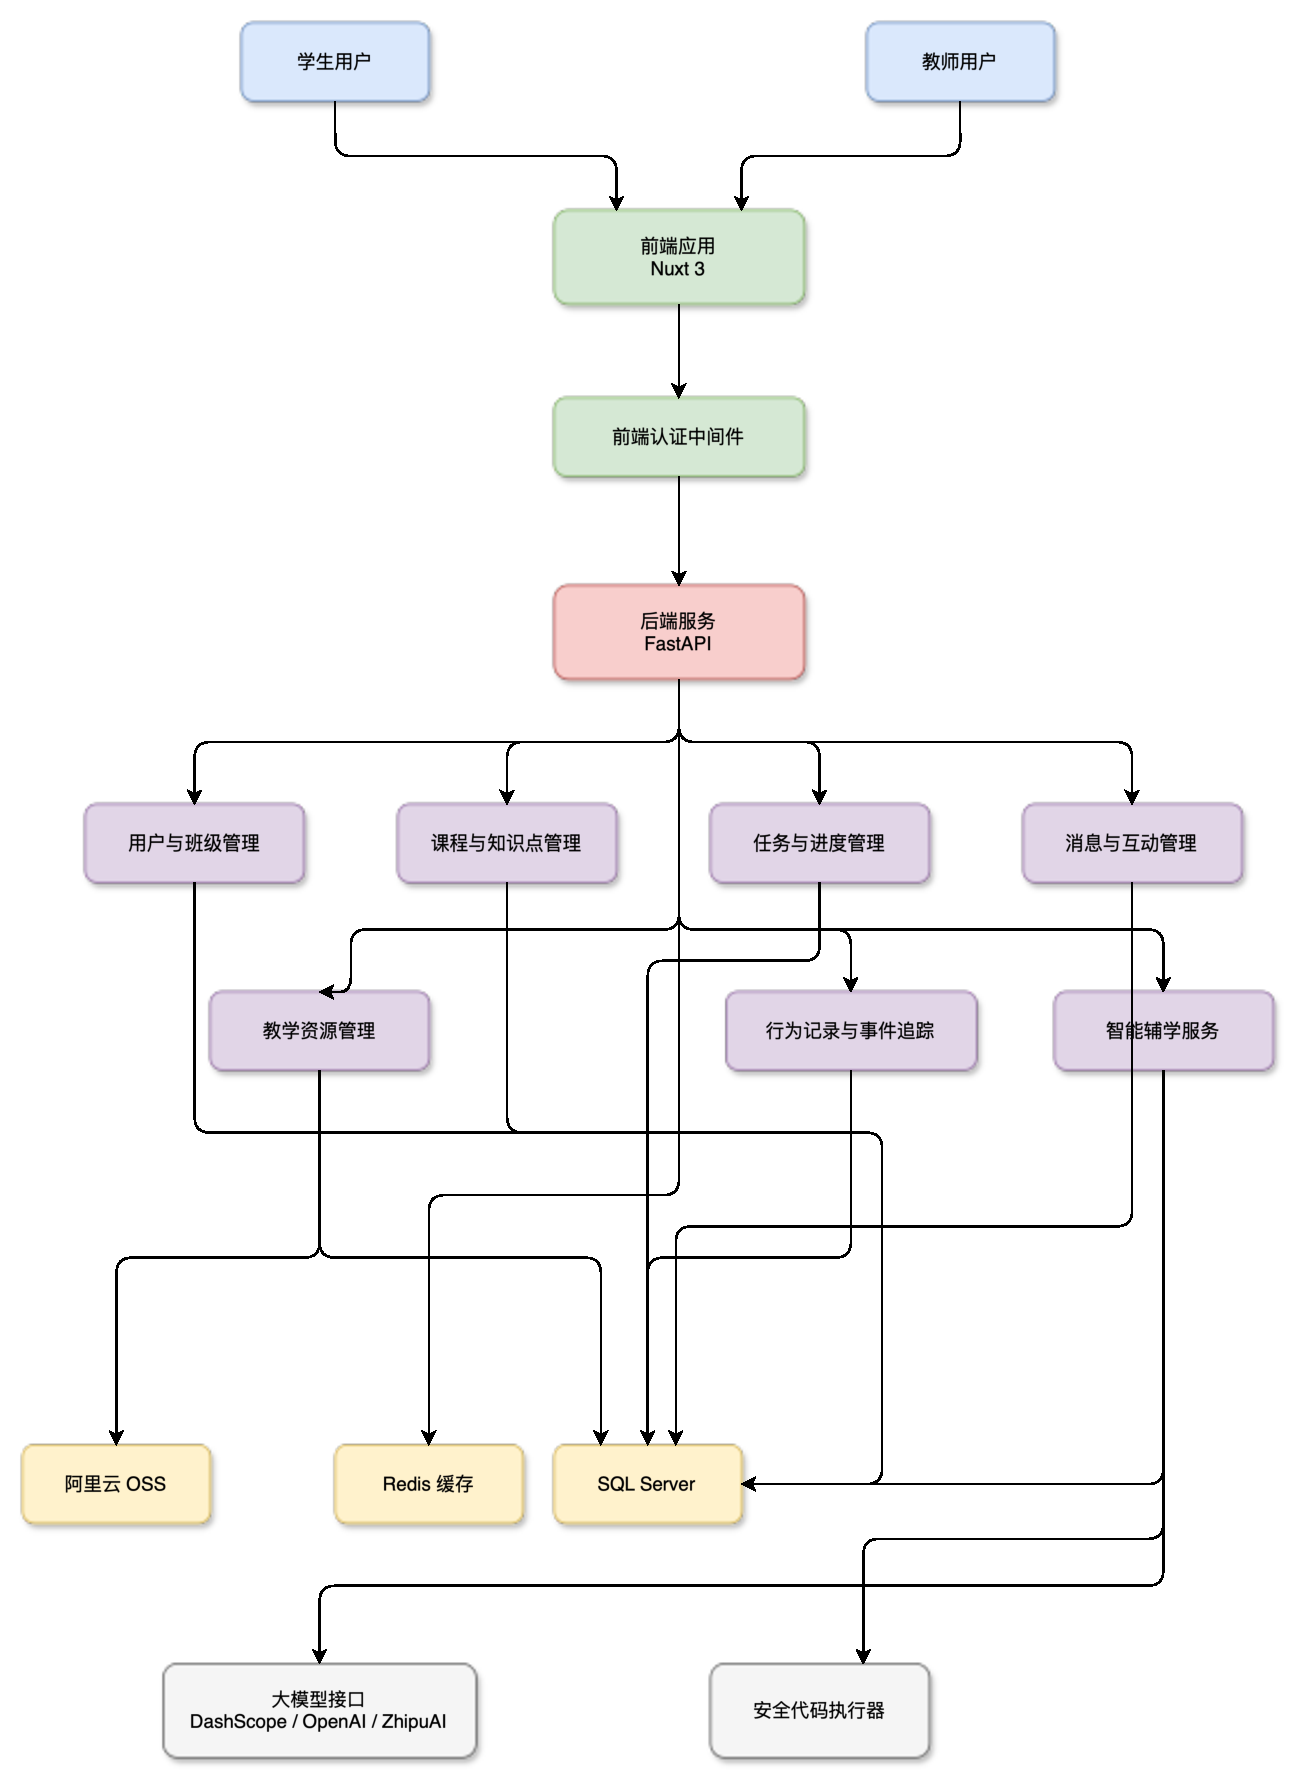
\includegraphics[width=0.9\textwidth,keepaspectratio]{figures/body/系统总体架构图.pdf}
  \caption{系统总体架构图}
  \label{fig:system-arch}
\end{figure}

该架构中，前端通过统一接口调用后端服务。后端会按业务域对请求进行分发，例如用户管理、课程管理、任务管理、消息互动、资源管理、行为记录与智能辅学等模块。智能辅学模块内部并不走单一链路：涉及自然语言与代码解释的请求通过大模型接口处理；在线代码运行与错误返回则由安全代码执行器完成。

\section{系统功能模块设计}
根据业务需求，平台功能可以划分为以下几个模块，如图~\ref{fig:system-modules}所示。

\begin{figure}[htbp]
  \centering
  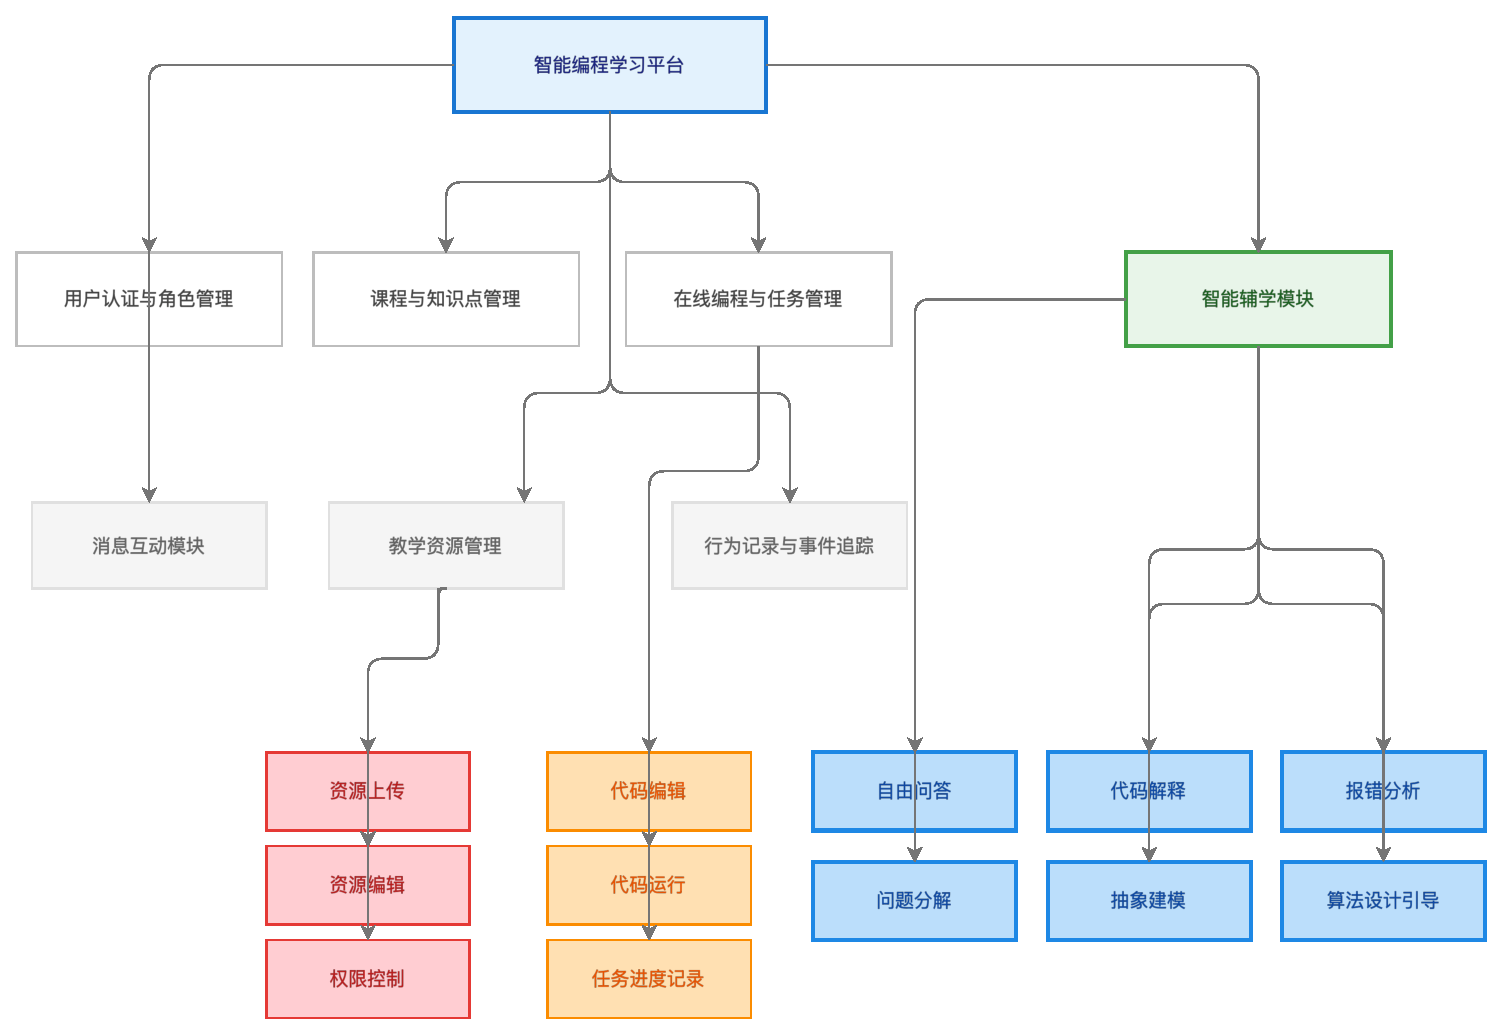
\includegraphics[width=0.9\textwidth,keepaspectratio]{figures/body/系统功能模块图.pdf}
  \caption{系统功能模块图}
  \label{fig:system-modules}
\end{figure}

\section{前后端结构设计}
\subsection{前端结构设计}
前端结构采用“页面 + 组件”的方式组织。页面层覆盖登录页、学生主页、教师主页等入口页面，并包含课程更新页、事件记录页与事件追踪页等业务页面。组件层主要沉淀可复用单元，例如课程分类选择器、课程搜索选择器、知识点选择器，以及聊天组件和富文本编辑器等。

在前端结构组织上，本文采用“页面承载业务、组件复用交互”的设计思路。页面层以流程编排为主，负责触发数据请求；组件层聚焦交互单元复用，并管理局部状态。这样划分后，不同业务页面的职责边界更容易保持清晰；在课程筛选、聊天交互与资源编辑等高频场景中，也能减少重复开发工作。

学生端页面更关注学习路径的长度，目标是尽量减少学生完成“查看课程—进入任务—编写代码—查看反馈”主流程时的页面跳转与操作负担。教师端页面则把重点放在内容维护效率与信息聚合能力上，课程编辑、任务配置、资源管理和学习记录查看等常用入口尽量集中在同一界面呈现。

\subsection{后端结构设计}
后端以路由模块组织业务接口，并通过统一认证依赖控制访问权限。公开接口主要用于登录与基础班级信息访问；其余接口在鉴权后开放，覆盖课程、任务、记录、资源、消息和点赞等模块。该结构有助于使路由职责更清晰、权限边界更明确，同时也为后续模块扩展留出空间。

在后端结构上，系统按业务域划分接口模块，使用户管理、课程管理、任务管理、资源管理、消息互动和学习记录等功能在相对独立的边界内演进。与按页面或按角色分散定义接口相比，这种方式更符合服务端对数据与业务规则统一管理的需求；当后续增加新模块时，也更有利于保持接口体系的连续性。

同时，后端结构设计还需要兼顾“通用能力集中化”和“业务能力解耦化”。认证校验、异常处理与统一返回格式等能力应尽量沉淀为公共机制，避免多个接口重复实现。课程维护、代码运行与智能辅学等业务逻辑则按模块分别组织，以降低彼此耦合。通过这种方式，系统既能保持整体一致性，也能保留业务扩展弹性，实现收放自如。


\chapter{系统详细设计}

\section{数据库设计}
\subsection{数据库概念结构设计}
系统数据库围绕用户、课程、任务、知识点、资源、评论消息、点赞关系和学习记录等核心实体展开。主要关系如图~\ref{fig:er-concept}所示。

\begin{figure}[htbp]
  \centering
  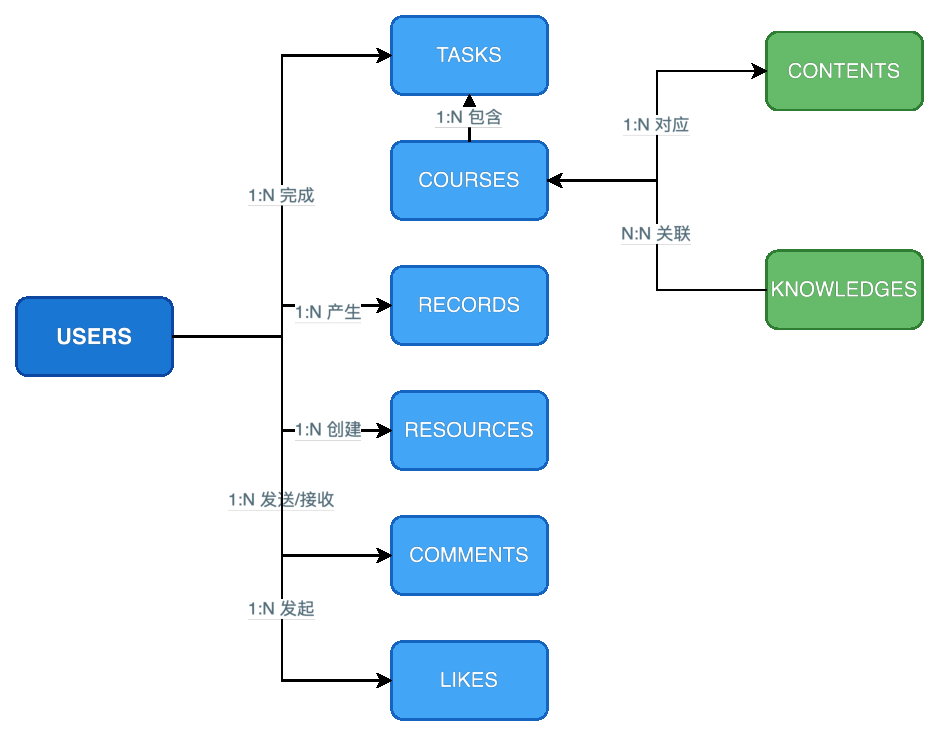
\includegraphics[width=0.9\textwidth,keepaspectratio]{figures/body/数据库概念结构图.pdf}
  \caption{数据库概念结构图}
  \label{fig:er-concept}
\end{figure}

从概念设计角度看，数据库结构并非仅为页面展示提供存储空间，而是承担整个平台业务关系表达的职责。用户实体连接学习行为与互动行为；课程实体连接知识点、任务与资源；记录实体承担学习过程留痕功能。这样的设计既能保存结果数据，也能保留过程数据，为后续统计分析与教学干预提供基础。

在概念模型的基础上，本文进一步细化各实体的属性与关联约束，得到如图~\ref{fig:er-logical}所示的系统数据库逻辑结构图（E-R 图）。该图描述了用户、课程、任务、知识点、资源、评论、点赞和学习记录等实体之间的主外键关系及业务关联，为后续主要数据表设计提供依据。

\begin{figure}[htbp]
  \centering
  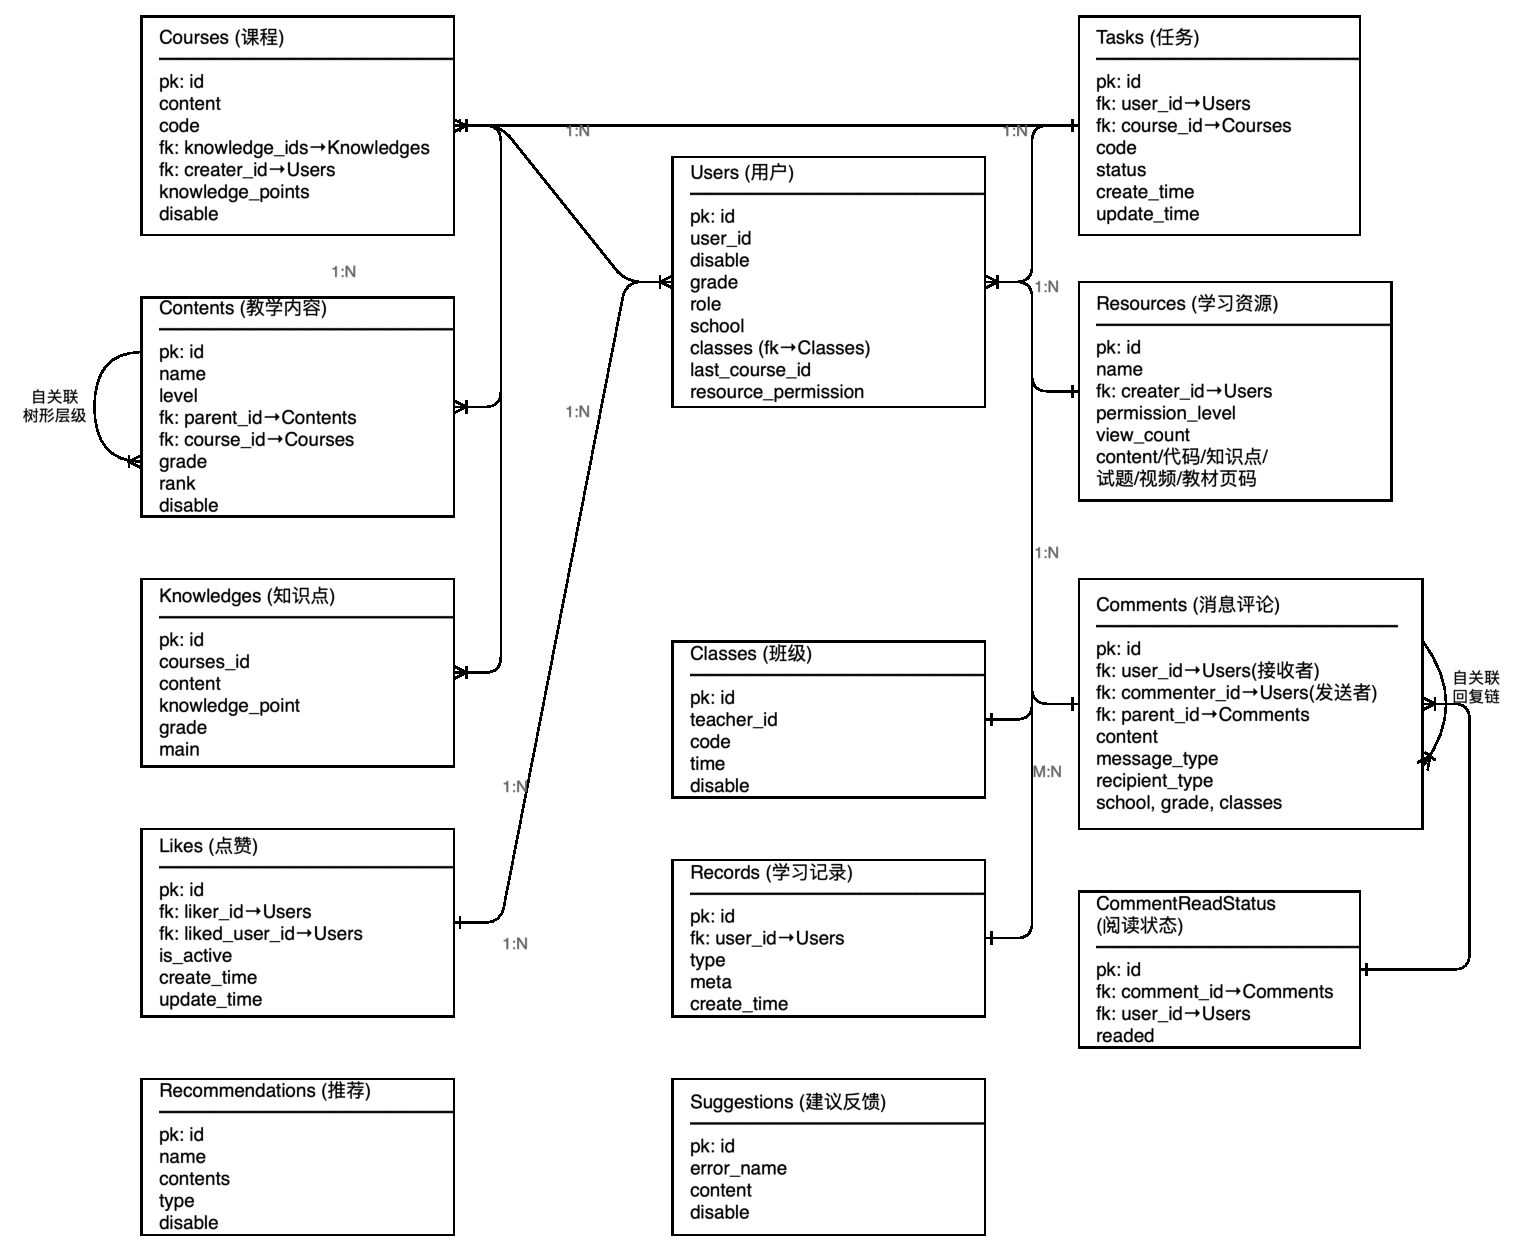
\includegraphics[width=0.9\textwidth,keepaspectratio]{figures/body/数据库逻辑结构图.pdf}
  \caption{系统数据库逻辑结构图（E-R 图）}
  \label{fig:er-logical}
\end{figure}

\subsection{主要数据表设计}
主要数据表设计如表~\ref{tab:database-tables}所示。

\begin{table}[htbp]
  \centering
  \caption{主要数据表设计}
  \label{tab:database-tables}
  \begin{tabular}{ll}
    \toprule
    数据表 & 说明 \\
    \midrule
    users & 存储用户基础信息、角色、学校、班级等 \\
    courses & 存储课程信息和课程内容索引 \\
    contents & 存储课程层级内容结构 \\
    tasks & 存储学生任务代码、状态与时间信息 \\
    knowledges & 存储知识点与内容关联信息 \\
    resources & 存储教学资源与权限信息 \\
    comments & 存储消息与评论内容 \\
    likes & 存储点赞关系 \\
    records & 存储学习行为和错误记录 \\
    \bottomrule
  \end{tabular}
\end{table}

在逻辑设计上，users 表是权限识别与角色管理的基础。课程内容组织由 courses、contents 与 knowledges 共同构成。tasks 表用于承载学生任务完成状态与代码提交结果，resources 表用于管理教学材料。互动关系通过 comments 与 likes 维持，而页面访问、代码运行和错误类型等过程数据则由 records 表记录。各数据表之间通过主外键关系或业务关联字段建立联系，从而支撑课程学习、任务执行和行为分析等核心流程。

数据库设计的关键不在于数据表数量多少，而在于业务语义是否清晰。若一个表承担过多职责，后续维护时就容易出现字段膨胀和语义混乱；若表之间关联关系过于松散，又会削弱数据利用价值。因此，本文在设计时尽量使每张表承担较明确的业务职责，并为后续扩展预留适当空间。

\section{智能辅学模块设计}
智能辅学模块的处理链路可概括为“提问输入”“场景识别”“提示词构造”“模型生成”和“结果返回”五个环节。面向不同学习任务，系统会分别调用自由问答、代码解释、报错分析、问题分解、抽象建模和算法设计等功能接口；其处理流程如图~\ref{fig:ai-tutor-flow}所示。

\begin{figure}[htbp]
  \centering
  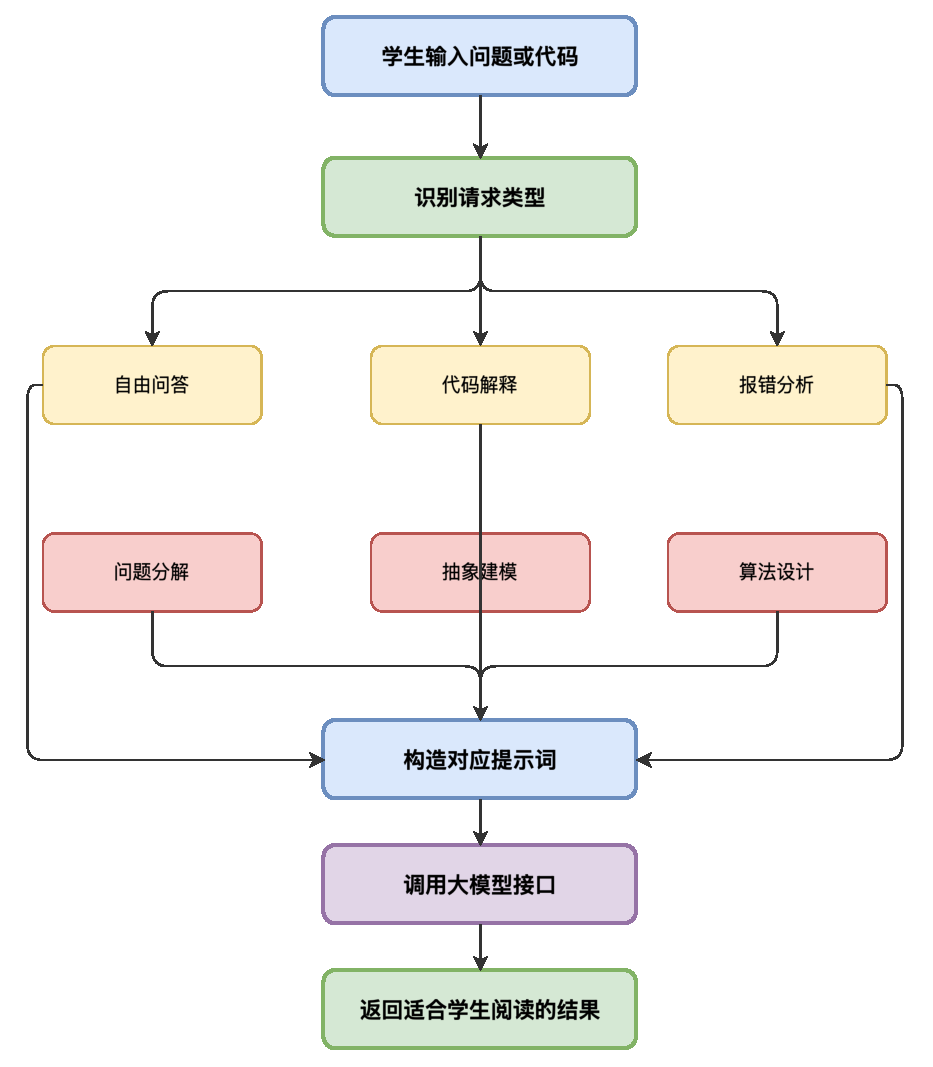
\includegraphics[width=0.9\textwidth,keepaspectratio]{figures/body/智能辅学模块处理流程图.pdf}
  \caption{智能辅学模块处理流程图}
  \label{fig:ai-tutor-flow}
\end{figure}

为避免大模型输出与教学目标脱节，本文进一步将该模块细化为“场景识别—约束生成—教学化输出—风险兜底”的四层结构。

在场景识别层，系统不将学生输入统一视为普通问答，而是结合问题文本、代码内容、运行结果和任务上下文，对请求进行类型划分，例如自由问答、代码解释、报错解析、问题分解、抽象建模和算法设计引导六类任务。其目标是让不同任务调用不同的提示模板与输出结构，避免模型在所有场景下采用同一种回答方式。

在约束生成层，系统将学生年级、课程主题、知识点标签、任务目标和回答边界写入提示内容\cite{tang2025middleschool,chen2025debugging}。本文强调两类约束：教学约束强调回答应当循序渐进、语言适龄，并避免无前提地直接给出完整答案；安全约束则要求拒绝危险代码、规避越权请求，并限制与课程目标无关的输出扩散。这一思路与现有研究中关于人在回路和教学对齐的观点一致\cite{ma2024teachableagent,pirzado2024pitfalls}。

在教学化输出层，系统不追求一次性给出最完整答案，而是优先保证回答的教学可用性。以报错解析为例，系统要求模型依次给出错误含义、错误位置、可能原因与修改建议。再如算法设计引导场景，系统要求模型先帮助学生明确输入、输出与关键步骤，再逐步组织流程。借助这种结构化输出，平台更容易将模型回答转化为学生能够理解和消化的学习材料，做到由浅入深、层层递进。

在风险兜底层，系统保留日志记录、人工复核与规则拦截机制。若出现高风险输出、低置信度回答或涉及完整作业答案的请求，平台会优先采用弱化回答、返回思路框架或提示教师介入等处理方式。该层并非附加功能，而是教育场景接入 LLM 的必要条件。缺少兜底机制的大模型，更像一辆制动不足的车，速度虽快，却难以稳妥驶入课堂。

\section{系统部署设计}
系统前端可通过 Node 环境进行 Nuxt 部署；后端侧通过 Uvicorn 运行 FastAPI 服务。数据库使用 SQL Server，缓存使用 Redis；静态资源与教学视频使用阿里云 OSS 进行存储。后续若需要提升服务稳定性，可进一步接入负载均衡和弹性伸缩机制。

从部署关系看，前端应用主要负责页面渲染与交互请求发起；后端服务负责接口处理与业务调度。数据库承担结构化数据持久化，Redis 负责部分高频数据缓存，OSS 则用于教学视频等非结构化资源存储。该部署方式能够较清晰地划分职责边界，避免所有压力集中到单一服务节点。

在毕业设计的实现规模下，上述部署方式已经能够满足系统演示和功能联调需求；若面向更大规模的教学使用，还需要进一步考虑服务容错、日志监控、备份恢复和并发调度等问题。部署设计就像搭建一座教学楼的管线系统，平时不显眼，但一旦规划混乱，后续所有功能都会受到牵连。论文中明确部署关系，有助于完整说明系统从设计到运行的落地路径。


\chapter{软件实现}

\section{用户认证与权限控制实现}
系统采用 JWT 作为用户认证机制。登录成功后，前端会持久化必要的用户状态，并借助全局认证中间件拦截需要登录权限的页面访问。后端侧则通过依赖注入完成身份校验，同时将公开接口与受保护接口分组管理。

认证模块的核心目标在于保证“用户身份可信”，并让“接口访问有边界”。学生与教师共用同一平台入口，但两类角色可访问页面与可执行操作并不相同。为此，系统在登录后不仅判断认证状态，也会读取角色属性，再据此决定可见菜单、可访问路由以及可调用接口范围。

前端侧主要负责维持登录态，并执行页面级拦截：用户完成登录后，系统保存必要的身份状态；页面切换时，先判断当前页面是否需要认证，从而在前端提前挡住未授权访问，减少无效请求进入后端。后端侧承担最终校验职责，通过统一认证依赖校验令牌有效性与用户身份，在关键接口中再进一步核对角色权限。

权限控制模块关注的不只是“谁能进来”，更关心“进来之后能做什么”。如果缺少细粒度权限边界，教师端的资源维护能力与学生端的学习操作就可能相互混淆，进而影响数据安全与系统秩序。因此，认证与权限控制虽然在界面上并不显眼，却是平台稳定运行的基础。

\section{课程与知识点管理功能实现}
平台通过课程分类选择器、课程搜索选择器与知识点选择器组织课程内容。教师可在课程更新页面完成课程内容编辑、知识点关联以及代码内容维护；前端借助富文本编辑器提升录入效率，后端负责课程与知识点数据的持久化。

课程与知识点管理模块的实现重点是内容结构化。若课程内容仅以零散条目呈现，学生学习时很难形成清晰的知识路径\cite{hwang2013conceptmap}，教师维护时也不易保证内容一致性。基于此，平台在课程、知识点与资源之间建立关联关系，使课程不仅用于展示，也承担知识组织与任务承载的基本职责。

在教师使用流程中，课程维护通常包含新增课程、编辑课程描述、关联知识点、补充示例代码以及调整内容顺序等操作。为降低维护成本，前端页面尽量将这些动作收拢到同一工作界面，减少教师在多个页面间来回切换。后端接收结构化表单数据，并保证课程与知识点的关联关系能够稳定写入数据库。

对学生而言，该模块的价值主要体现在“看得懂课程结构”以及“找得到对应内容”。课程模块设计是否合理，会直接影响后续任务管理、智能问答与资源推荐等模块的使用体验。课程结构清晰，后续功能才有稳定落点；结构若混乱，即使其他模块功能完善，也容易被用成零散工具。

\section{在线编程与代码运行功能实现}
在线编程功能是系统核心模块之一。学生提交代码后，后端先完成语法检查，再执行安全检查；两项检查通过后，由安全执行器负责实际运行。系统会将执行结果或错误信息返回前端，并把运行行为写入数据库。其主要流程如图~\ref{fig:code-run-flow}所示。

\begin{figure}[htbp]
  \centering
  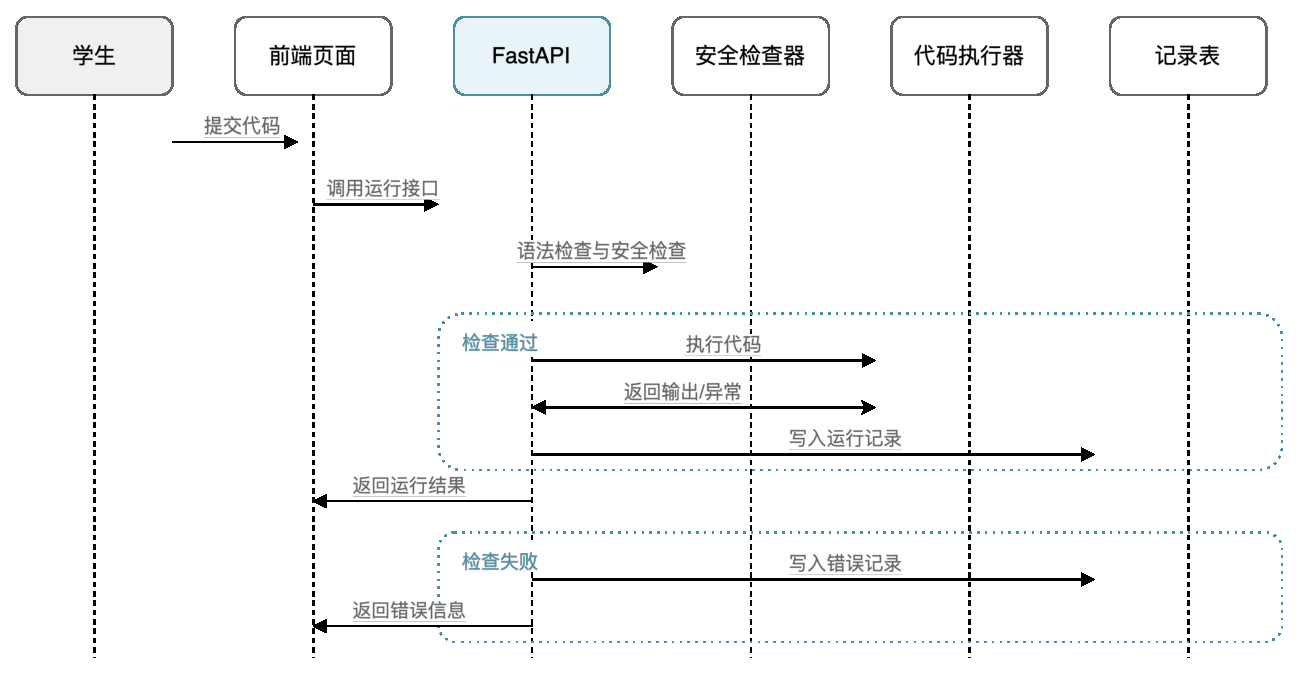
\includegraphics[width=0.9\textwidth,keepaspectratio]{figures/body/在线编程与代码运行流程图.pdf}
  \caption{在线编程与代码运行流程图}
  \label{fig:code-run-flow}
\end{figure}

从实现逻辑看，在线编程与运行流程大致经历四步：输入接收、静态检查、受控执行与结果回传。输入接收用于统一收集学生代码、任务标识与运行参数；静态检查侧重识别语法错误、危险导入和高风险函数调用；受控执行在限定环境中运行代码，并监控运行时长与输出规模；结果回传则把标准输出、异常信息或检查失败原因反馈到前端页面。

其中，静态检查与受控执行属于关键环节。代码接收后若直接执行，平台稳定性会与服务器安全性都会承担较大风险；反过来，若系统仅返回“运行失败”而缺少清晰原因，也难以满足教学场景的反馈需求。因此，本平台在设计上同时兼顾两点：控制执行边界，并保留教学所需的反馈信息。前者用于兜住安全问题，后者用于支撑学习过程，两者缺一不可。

此外，代码运行模块还承担行为记录功能。每一次运行请求，无论成功与否，都可能折射学生的学习状态：同类语法错误反复出现，往往意味着相关知识点尚未真正掌握；某一任务若长时间停留在运行失败，也可能说明学生在任务分解阶段已经遇到困难。因此，代码运行结果既服务于当前页面反馈，也为教师后续分析学生学习过程提供数据基础。

\section{大模型辅助教学功能实现}
\subsection{自由问答功能实现}
系统为编程相关问题提供流式问答能力。为限制回答范围并贴合学生使用场景，后端在请求发送给模型前加入系统提示词，用于约束回答主题与回复方式。

在该功能中，系统不把模型简单视为开放聊天接口，而是通过提示约束将其限定在编程学习支持场景内。模型回答的重点放在概念解释、思路提示与学习引导上，避免生成与课程无关的泛化内容，从而降低偏离教学目标的概率。

进一步地，相关研究表明，结构化且可回合追踪的同伴对话反馈机制有助于促进深度学习过程中的反思与策略修正\cite{yao2022dialogue,li2023trust}。据此，本文在自由问答实现中强调问题澄清、分步追问与关键点回收，尽量避免一次性长答案挤占学生的自主思考空间。

\subsection{代码解释功能实现}
代码解释功能以学生提交的代码为输入：模型先概括程序整体功能，再逐步解释关键语句，帮助学生形成从整体到局部的理解路径。

本文在该功能设计中更强调解释顺序而非解释长度。对于初学者而言，若系统一开始就逐行解释所有细节，学生往往会陷入局部信息而失去整体把握。基于这一点，本平台优先要求模型先说明程序“在做什么”，再说明“为什么这样做”，随后进入关键语句解释。这种组织方式更符合中小学生由整体到局部的理解路径。

\subsection{报错解析功能实现}
报错解析功能会同时接收学生代码与运行输出，并通过提示词约束模型采用“三步式”输出：先解释错误含义，再定位错误位置，最后给出启发式修改引导。这种组织方式更适合中小学生编程学习中的循序渐进式反馈。

与直接展示原始报错信息相比，报错解析功能更强调“翻译”与“拆解”。不少初学者并不是完全不能改错，而是读不懂错误信息，也说不清应先看哪一行、先改哪一步。因此，系统在此处引入结构化输出，并非为了增加模型参与感，而是为了把原本碎片化、技术化的报错信息转写为学生能够操作的修改线索。

\subsection{问题分解功能实现}
系统根据课程内容与学生任务描述，把复杂编程任务拆分为若干可执行步骤，以降低问题理解难度。

问题分解功能主要面向综合任务场景。学生面对较长任务描述时，常会出现“不知道从哪里开始”的情况。对此，系统不直接替学生完成程序，而是将任务拆分为输入分析、数据处理、条件判断、循环组织与结果输出等步骤，让学生先找到入口，再逐步推进实现过程。

\subsection{抽象建模功能实现}
系统通过抽象建模功能引导学生从具体问题中提炼一般规律，帮助其建立更稳定的问题求解方式。

这一功能的重点不在于给出标准模型，而在于帮助学生完成“从具体到一般”的过渡。中小学生编程学习中常见的情况是：在单个例题里能够模仿做法，但很难把方法迁移到相似问题。抽象建模功能的价值，就在于提炼输入对象、处理规则与输出目标，帮助学生逐步形成可迁移的思维框架。

\subsection{算法设计引导功能实现}
算法设计引导功能通过“开始、输入、处理、循环、输出、结束”等模板提示学生组织思路，帮助其逐步形成结构化的算法表达能力。

在实现上，该功能更接近思路支架，而非答案生成器。系统用固定过程模板帮助学生组织解题步骤：先明确流程结构，再进入代码表达阶段。这样做的目的，是把原本容易混乱的解题过程拆成可检查的步骤链条，从而降低学生在编码前的思维混乱程度。

\section{师生互动与消息功能实现}
平台通过评论消息相关接口实现师生之间以及学生之间的互动。系统支持消息发送、消息读取、未读状态管理和对话内容展示，可用于课后答疑与学习交流。

消息模块的实现意义在于补足教学平台中的“人际反馈链路”\cite{yao2022dialogue,li2023trust}。如果平台只有课程、任务和模型回答，而缺少教师与学生之间的直接互动，那么许多需要情境判断和个别化解释的问题仍然难以得到有效处理。因此，消息模块并不是对智能功能的重复建设，而是对其必要补充。

在具体实现中，系统需要同时处理消息内容、发送关系、接收状态与未读标记等信息，使互动过程既可追踪又便于管理\cite{li2023trust}。对教师而言，消息模块能够承载课后答疑与个别提醒；对学生而言，则能够在模型回答不足或需要确认任务要求时，保留向教师继续求助的正式通道。

\section{教学资源管理功能实现}
教师端可对教学资源进行创建、修改、删除和权限设置。资源信息包括名称、内容、代码、教材页码、视频链接和知识点标签等，用于支撑课堂教学与课后扩展学习。

教学资源管理模块的重点在于资源与教学内容之间的可关联性。若资源只以文件形式独立存在，其教学价值往往取决于教师额外解释；若资源能够与课程、知识点和任务建立对应关系，学生在学习过程中就更容易找到“当前问题对应的辅助材料”。因此，本平台中的资源管理并非简单文件上传，而是面向教学组织的资源编排。

此外，资源权限设置也具有实际意义。部分资源适合全体学生查看，部分资源则更适合作为教师备课材料或分层教学补充内容。通过权限控制，平台能够在同一资源体系内兼顾公开学习支持与教师内部管理需求，从而提高资源复用效率。

\section{学习行为记录与事件追踪功能实现}
系统会记录用户学习过程中的页面访问、代码运行、错误类型等行为数据，并通过可视化页面展示学习记录与交互情况，为教师掌握学生学习进度与错误分布提供数据支撑。

从平台价值角度看，学习行为记录模块相当于系统的“观察窗”。若缺少该模块，平台虽然能提供教学功能，却很难回答“学生到底如何使用这些功能”这一关键问题。通过记录页面访问、代码运行、错误类型与交互过程，系统可以把原本不可见的学习过程转化为可分析的数据线索。

学习行为记录模块的意义不仅在于统计，更在于为后续教学干预提供依据。教师可依据行为数据识别高频错误知识点，判断哪些任务难度偏高，或发现哪些学生长期缺乏有效互动。对毕业设计而言，该模块也为后续研究者引入学习者建模、分层推荐与教学效果评价提供了基础数据入口\cite{tsai2021cts}。

\section{系统界面展示}
本节通过系统运行截图，对平台主要用户界面进行展示与说明。

\subsection{登录界面}
图~\ref{fig:login}展示了系统的登录界面。整体采用居中卡片式布局，顶部"请登录"标题简明扼要。表单区域包含两个输入字段：账号输入框与课程码输入框，其中课程码字段在输入时以密码掩码显示，这一设计考虑了课堂环境中多人在场的使用场景，避免邻座学生窥视。蓝色主色调的登录按钮负责触发JWT令牌获取与前端状态持久化逻辑。对于尚未创建班级的教师用户，界面还提供了绿色的"生成课程码"按钮，点击后系统调用后端接口生成唯一课程码并回显，同时提供一键复制功能，便于教师快速将课程码分发给学生。登录成功后，系统读取用户角色字段并自动路由至对应主页：学生进入资源页，教师进入管理页。

\begin{figure}[htbp]
  \centering
  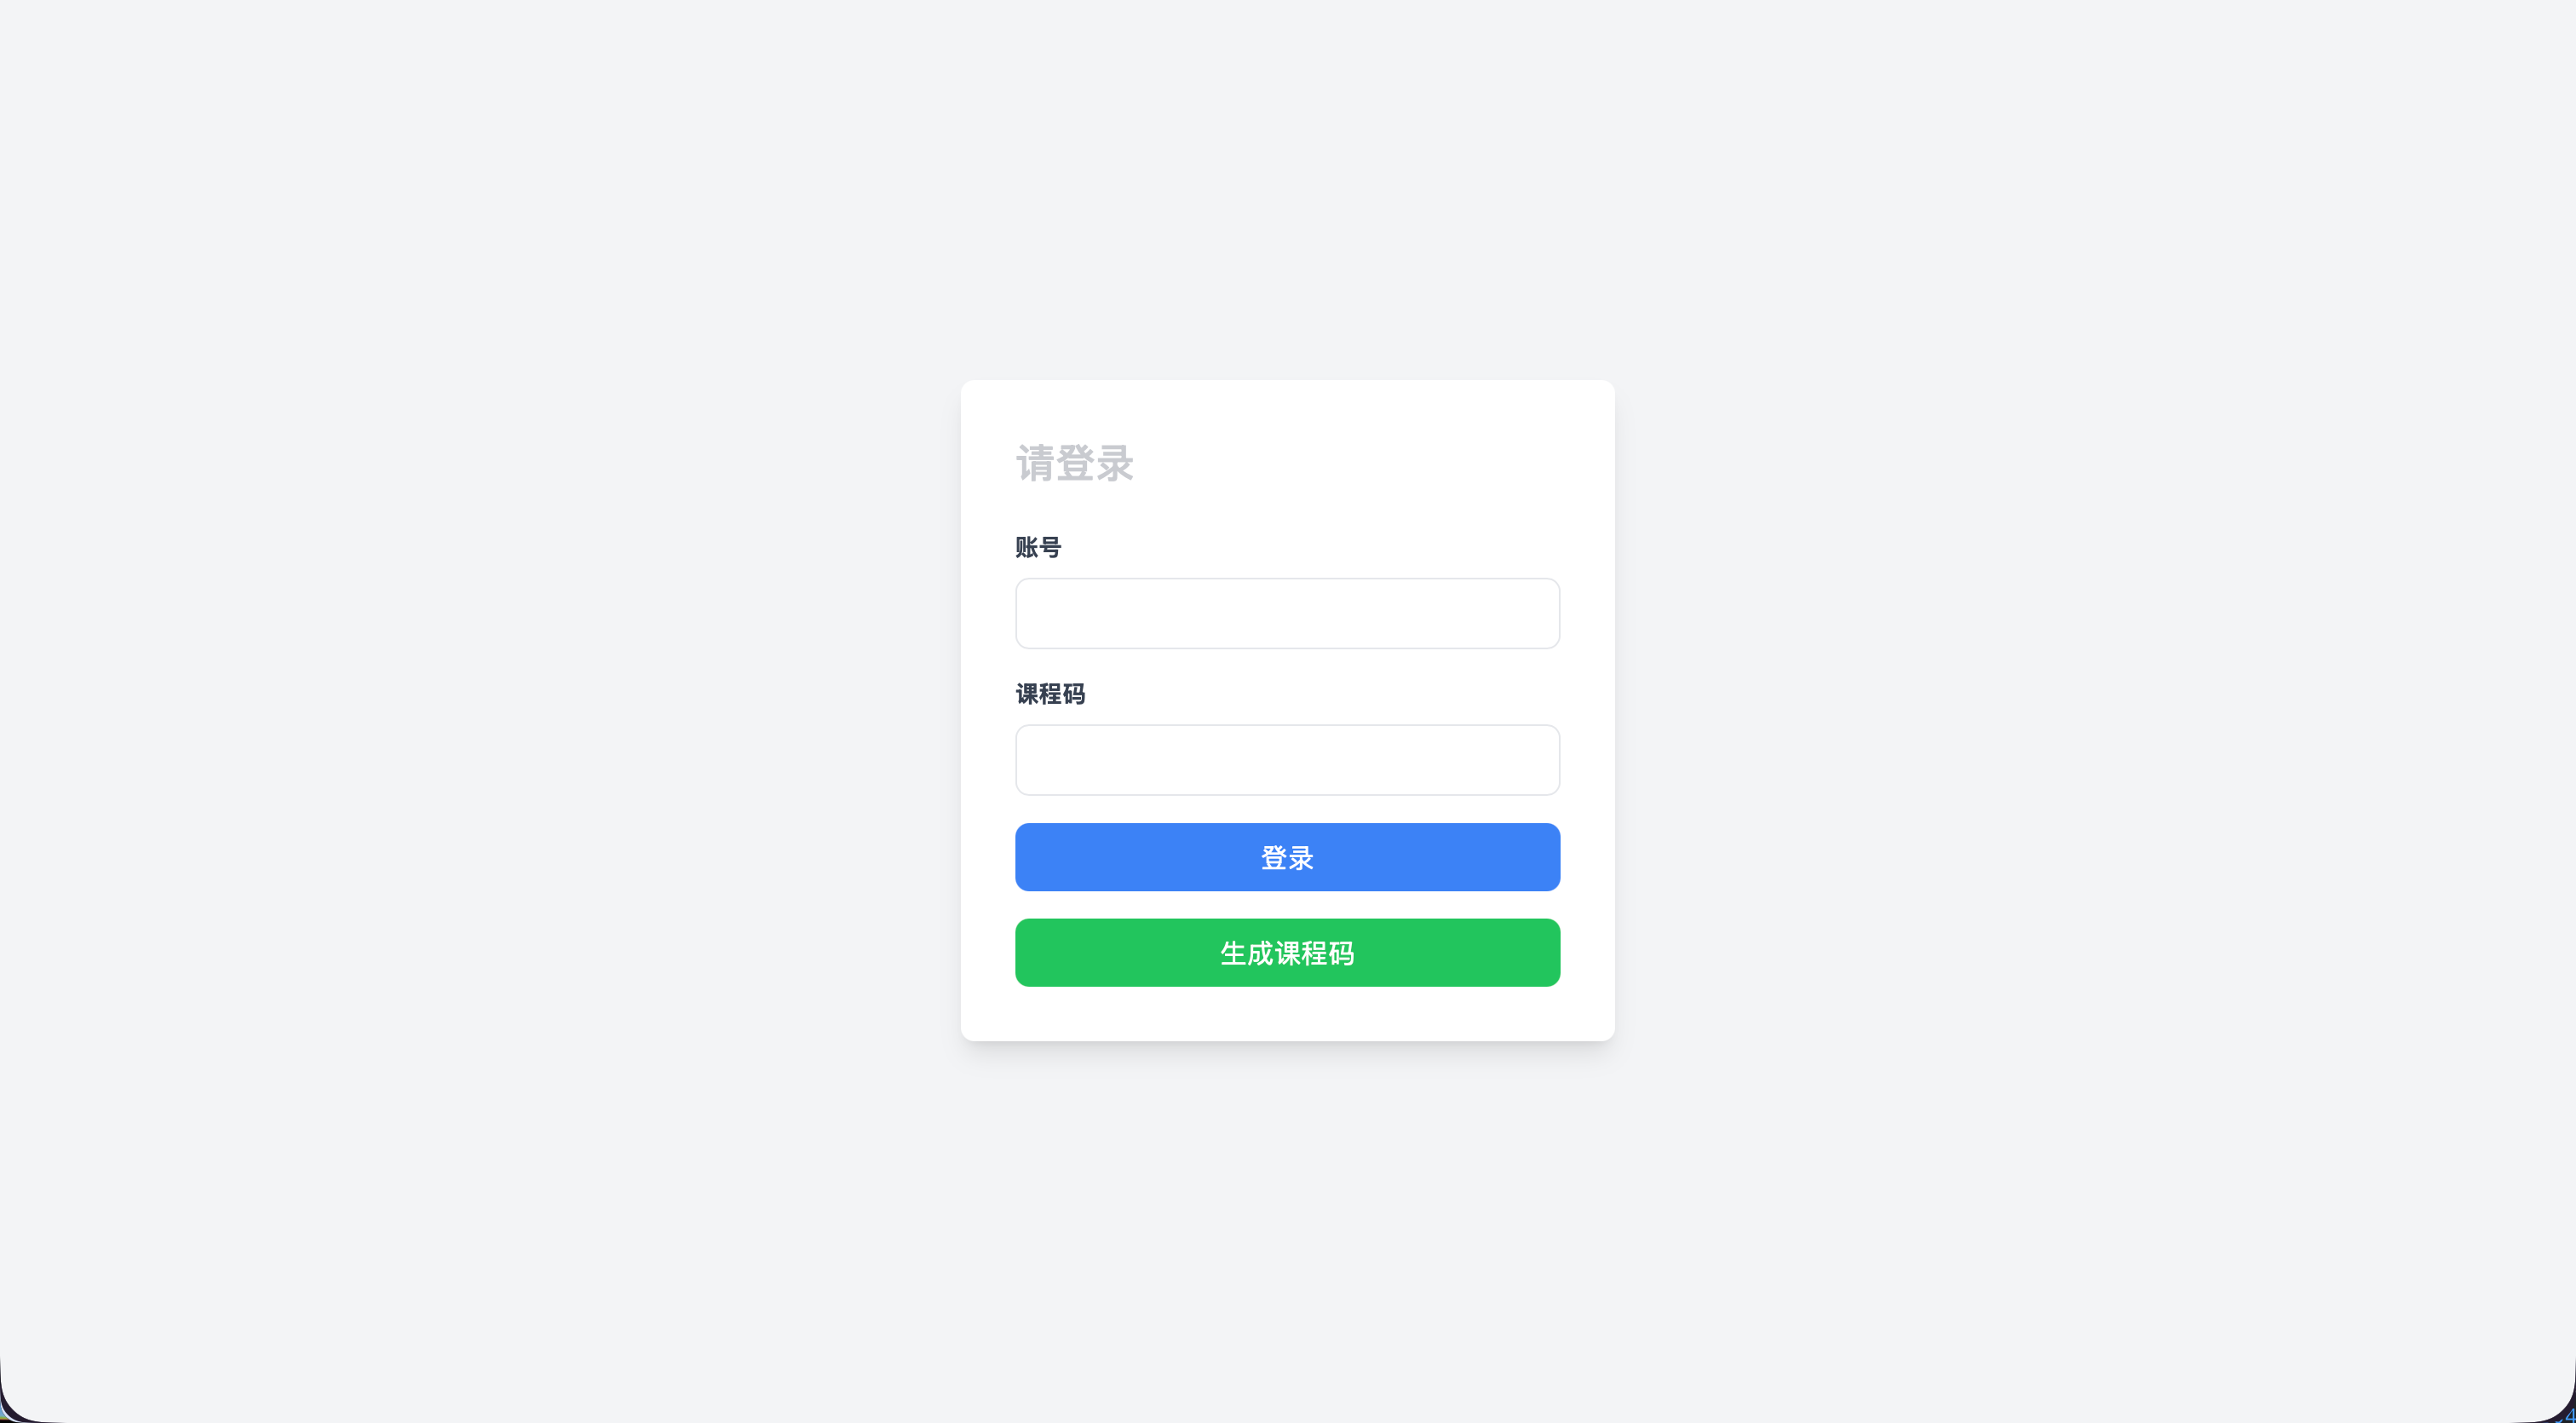
\includegraphics[width=0.5\textwidth,keepaspectratio]{figures/body/login.png}
  \caption{系统登录界面}
  \label{fig:login}
\end{figure}

\subsection{学生资源页仪表板}
学生端主界面采用 2×2 网格布局，将核心学习信息组织为四个功能区域，如图~\ref{fig:student-dashboard}所示。左上角的课程进度区域以表格形式呈现全班同学的完成情况，并标注个人完成率，学生可直观了解自己在班级中的相对位置，该区域还支持对同学进行点赞互动。右上角区域统计典型错误类型，系统根据学生的代码运行记录分析错误分布，并以水平进度条可视化各类错误的出现频率，这种设计帮助学生快速识别自身的高频错误模式。

左下角区域分为左右两部分：左侧为学习笔记面板，学生可在此记录学习心得；右侧为系统推荐的教学资源，内容包含教材页码与视频链接，点击即可跳转观看，观看结束后系统还会弹出满意度评价问卷以收集反馈。右下角为留言板区域，学生可搜索并查看同班同学列表，选择特定对象或切换至全班通知模式后发送留言，消息气泡根据发送者角色以不同颜色区分，便于快速识别对话来源。

\begin{figure}[htbp]
  \centering
  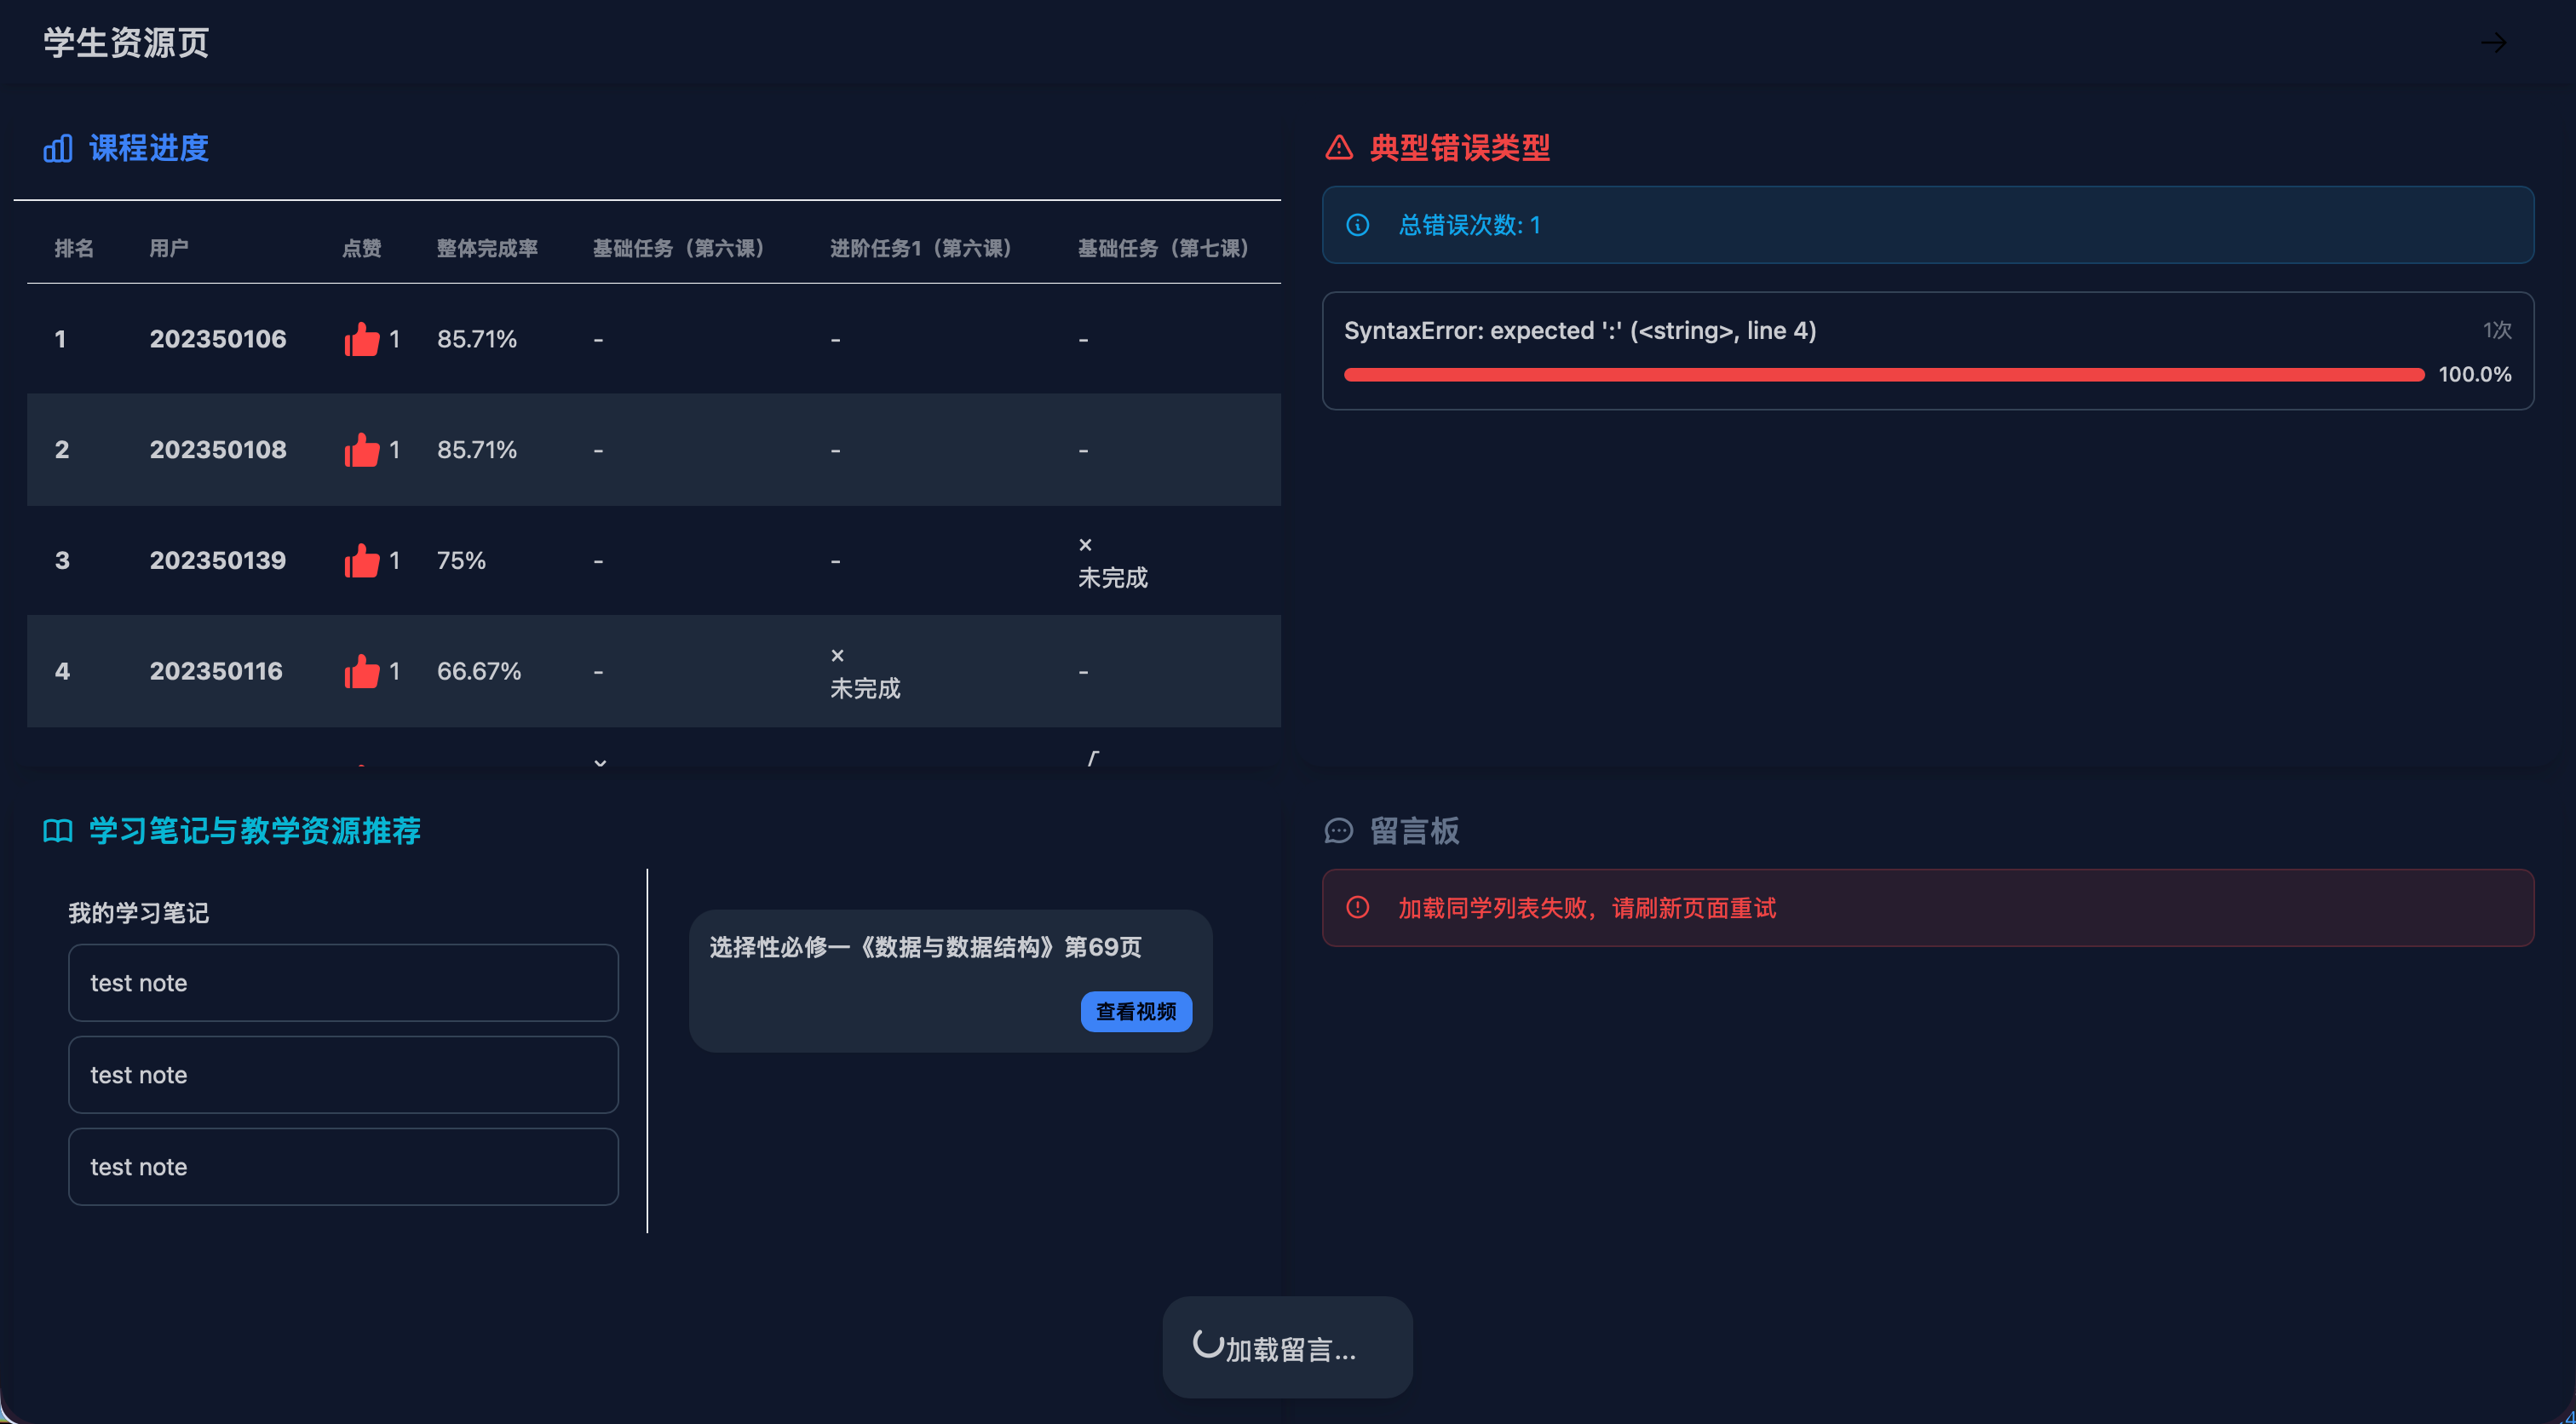
\includegraphics[width=0.9\textwidth,keepaspectratio]{figures/body/student_dashboard.png}
  \caption{学生资源页仪表板}
  \label{fig:student-dashboard}
\end{figure}

\subsection{教师资源页仪表板}
教师端采用上下分区布局，如图~\ref{fig:teacher-dashboard}所示。上半部分的全班学习进度表格采用虚拟滚动技术，即使班级人数较多也能保持流畅交互，表格中每名学生的各课程完成状态以√/×标记，并汇总整体完成率；教师可按学校、年级、班级维度进行筛选，快速定位需要关注的学生。下半部分采用左右分栏结构：左侧面板以百分比进度条展示班级典型错误分布，帮助教师把握整体错误特征；右侧为学习记录面板，教师可搜索学生列表、查看历史消息记录，并以教师身份发送回复、留言或通知，未读消息数量会在学生列表中实时提示。

\begin{figure}[htbp]
  \centering
  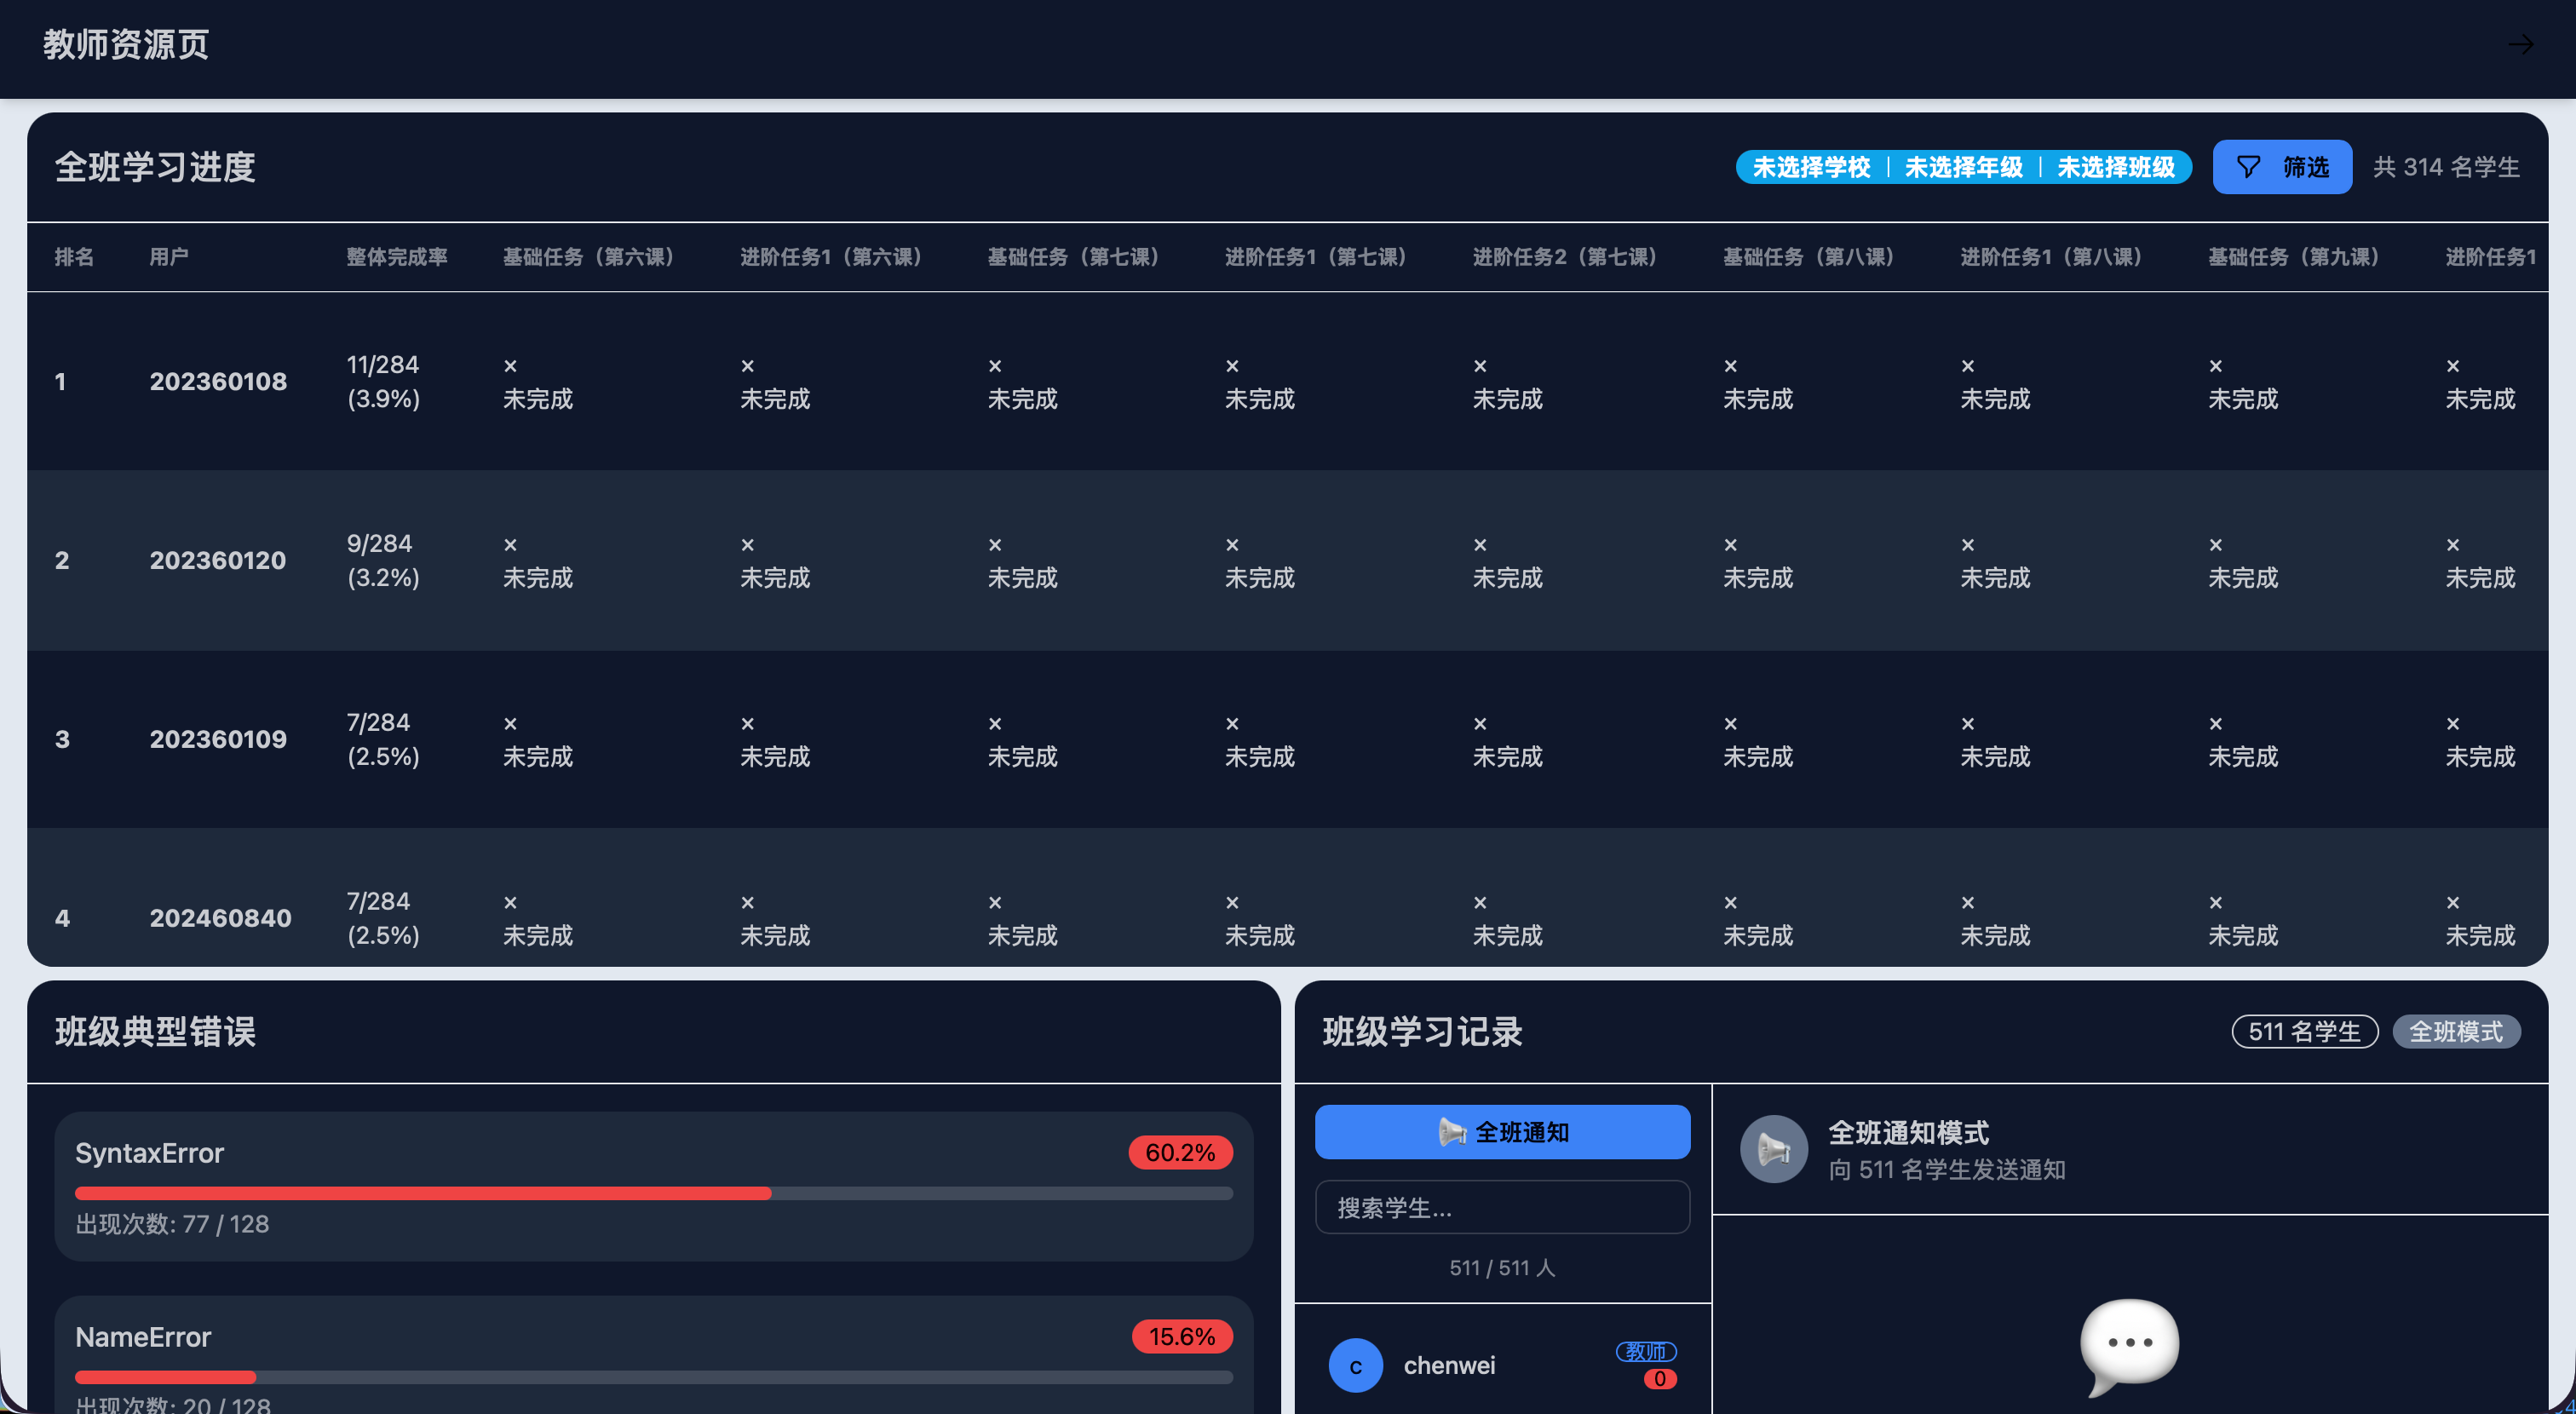
\includegraphics[width=0.9\textwidth,keepaspectratio]{figures/body/teacher_dashboard.png}
  \caption{教师资源页仪表板}
  \label{fig:teacher-dashboard}
\end{figure}

\subsection{教师资源管理页面}
教师在资源页可通过标签页切换至"教学资源"板块，如图~\ref{fig:teacher-resource}所示。该板块提供"所有资源"与"我的资源"两个视图：前者展示当前权限范围内可见的全部教学资源，后者仅展示教师本人创建的资源，这种区分便于教师快速定位自己维护的内容。每个资源卡片展示名称、关联知识点、权限级别（所有人/本学校/仅班级）、创建者、观看次数与创建时间等元信息。

教师可通过"添加资源"按钮创建新资源，填写名称、示范题目、资源代码、教材页码、视频链接与知识点后保存。对于已创建的资源，教师还能执行编辑或删除操作。资源权限级别由前端统一选择器控制，系统据此过滤不同权限的资源可见范围，从而实现分层教学资源的精细化管理。

\begin{figure}[htbp]
  \centering
  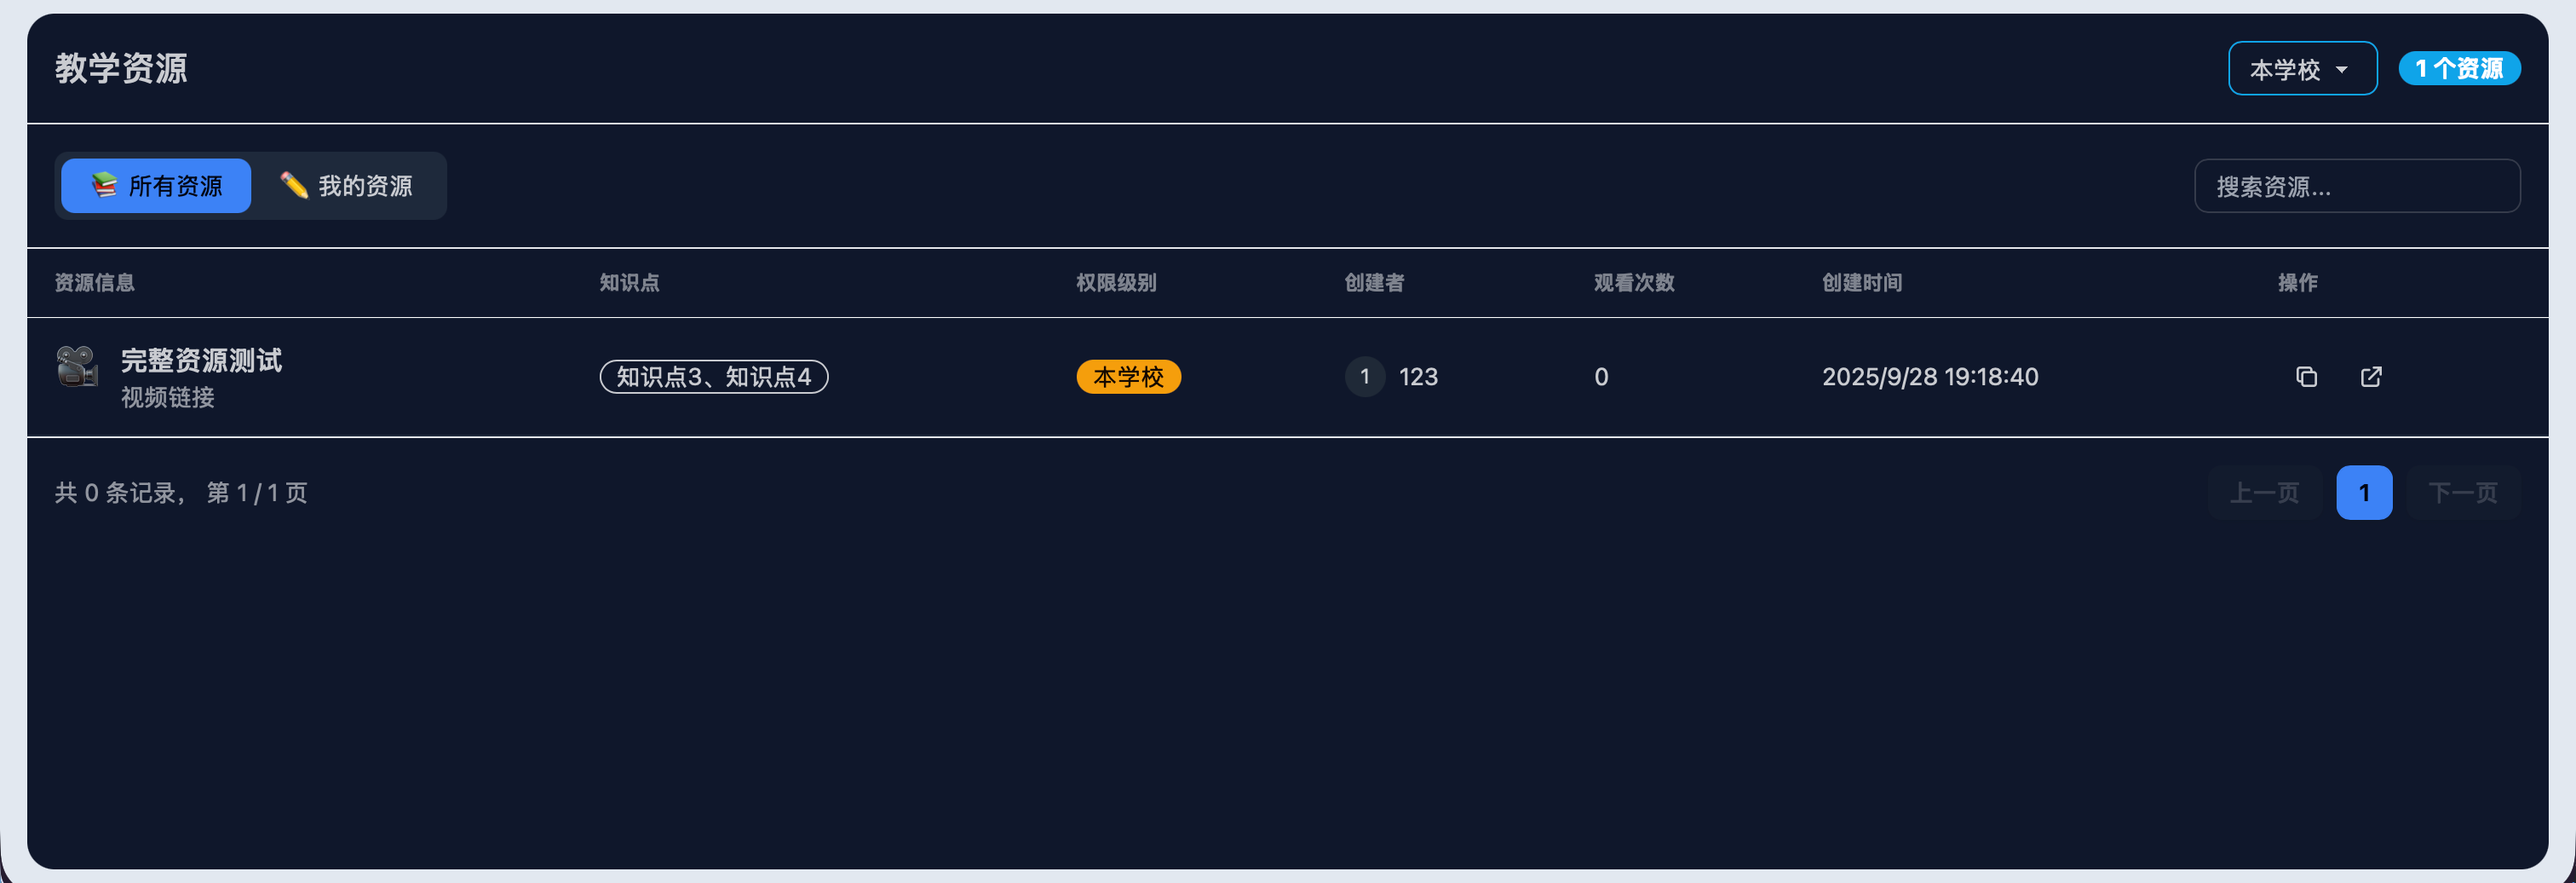
\includegraphics[width=0.9\textwidth,keepaspectratio]{figures/body/teacher_resource.png}
  \caption{教师资源管理页面}
  \label{fig:teacher-resource}
\end{figure}

\chapter{系统测试与调试}

\section{测试环境}
测试环境配置如表~\ref{tab:test-env}所示。

\begin{table}[htbp]
  \centering
  \caption{测试环境配置}
  \label{tab:test-env}
  \begin{tabular}{ll}
    \toprule
    类别 & 配置 \\
    \midrule
    前端环境 & Nuxt 3 + Node.js (pnpm) \\
    后端环境 & FastAPI + Python 3.14 + Uvicorn \\
    数据库 & SQL Server + SQLAlchemy ORM \\
    缓存 & Redis \\
    模型接口 & DashScope (通义千问) + OpenAI + 智谱 GLM \\
    对象存储 & 阿里云 OSS \\
    部署服务器 & 8 核 16G (生产环境) \\
    \bottomrule
  \end{tabular}
\end{table}

测试环境配置以贴近真实部署为目标，使测试结果具备实际参考价值。前端侧通过 ESLint 实施代码规范检查，构建过程启用 TypeScript 严格模式，以保障类型安全与重构可控性。后端服务则以 pytest 作为回归测试框架，逐层验证接口处理、权限校验与业务调度逻辑。数据库与缓存组件重点承担数据读写验证任务，尤其关注高频访问场景下的系统稳定性。模型接口测试则聚焦智能辅学链路，在实际调用中检验响应完整性与教学可用性。

本章测试并不只关注单个接口能否返回成功状态，而是围绕“登录认证—课程访问—代码提交—行为记录—教师反馈”这一学习闭环展开。后端自动化测试主要使用 SQLite 与 FakeRedis 构造轻量测试环境，避免测试过程依赖外部 SQL Server 与 Redis 服务；前端验证则结合构建检查、页面截图和浏览器控制台日志，判断界面渲染、路由跳转与接口调用是否符合预期。对于大模型相关功能，考虑到远程模型接口存在网络波动和服务排队等因素，测试重点放在请求链路、提示词选择、输出格式约束和异常兜底，而不简单以单次响应时长作为唯一依据。

\section{功能测试}
功能测试覆盖系统核心业务模块，测试结果如表~\ref{tab:func-test}所示。

\begin{table}[htbp]
  \centering
  \caption{功能测试结果}
  \label{tab:func-test}
  \begin{tabular}{cp{3cm}p{4cm}p{3cm}p{3cm}}
    \toprule
    测试编号 & 测试模块 & 测试内容 & 预期结果 & 实际结果 \\
    \midrule
    T1 & 登录认证 & 教师账号密码登录 & 登录成功并返回 JWT & 通过 \\
    T2 & 登录认证 & 学生错误课程码登录 & 返回 403 禁止访问 & 通过 \\
    T3 & 登录认证 & 未登录访问受保护接口 & 返回 401 未授权 & 通过 \\
    T4 & 在线编程 & 提交正确代码 \texttt{print(1+1)} & 返回输出 \texttt{2} & 通过 \\
    T5 & 在线编程 & 提交危险代码 \texttt{import os} & 返回 SecurityError & 通过 \\
    T6 & 在线编程 & 提交无限循环代码 & 返回迭代次数超限错误 & 通过 \\
    T7 & 报错分析 & 提交含语法错误的代码 & 返回错误解释与定位 & 通过 \\
    T8 & 消息互动 & 教师发送消息给学生 & 学生可正常接收 & 通过 \\
    T9 & 消息互动 & 查询师生对话记录 & 返回完整对话历史 & 通过 \\
    T10 & 资源管理 & 更新资源访问权限级别 & 权限更新成功 & 通过 \\
    T11 & 资源管理 & 查询资源权限设置 & 返回当前权限值 & 通过 \\
    T12 & 课程管理 & 访问课程内容接口 & 返回课程结构数据 & 通过 \\
    \bottomrule
  \end{tabular}
\end{table}

功能测试基于 pytest 框架编写，后端测试覆盖认证、权限控制、在线编程执行、消息互动与资源管理等多个模块。测试过程中借助 FastAPI 内置的 \texttt{TestClient} 发起接口调用，并在每次测试前完成登录态模拟，以此验证鉴权机制的有效性。

功能测试的组织围绕核心业务链路设计，避免陷入零散的界面点击检查。每项测试既验证单点功能可用性，也追溯前后流程的闭环完整性。以在线编程模块为例：确认代码可执行只是入口条件，后续还需核对运行记录是否准确写入数据库、错误信息是否按约定格式返回，以及前端页面能否正确解析并展示这些结果。

从测试脚本对应关系看，认证类用例主要落在 \texttt{test\_auth\_and\_permissions.py} 中，覆盖教师登录、学生课程码校验、未登录访问拦截和登录后身份检查；在线编程用例集中在 \texttt{test\_platform\_run.py}，分别验证正常输出、危险导入拦截和无限循环限制；消息与资源权限相关验证则由 \texttt{test\_comments\_and\_resources.py} 承担。这样的拆分方式与系统模块边界基本一致，便于在某一类功能发生修改后执行定向回归测试。

危险代码执行测试体现了系统在多层安全防护上的设计。首先通过 AST 语法树分析，检查代码中是否存在危险导入（如 \texttt{os}、\texttt{sys}、\texttt{subprocess} 等模块）；其次在执行过程中使用 \texttt{sys.settrace} 监控迭代次数，防止无限循环占用服务资源。测试结果表明，这两种机制均能有效拦截危险代码。

智能辅学功能的测试重点在于输出结构的规范性，而非仅仅确认模型"返回了内容"。在教育场景中，模型作答是否切题、条理是否清晰，以及能否适配中小学生的认知水平，都是必须纳入考量的维度。测试覆盖了自由问答、代码解释、报错解析、问题分解、抽象建模和算法设计引导六种场景，验证了系统提示词约束与输出格式机制的有效性。

\section{前端构建与代码质量检查}
前端项目以 pnpm 作为包管理器，通过 ESLint 实施代码规范检查。构建配置启用 TypeScript 严格模式，以保障类型安全与重构可控性。

执行 \texttt{pnpm run build} 后，系统成功完成生产版本构建，输出文件总大小约 137 MB（压缩后约 31.8 MB）。构建产物包含服务器端渲染所需的 Nitro 服务器文件，以及各页面的按需加载分块。

代码质量检查发现部分组件存在未使用变量、事件未声明等问题，主要集中在 \texttt{Chat.vue}、\texttt{KnowledgePointSelector.vue} 等组件中。这些问题属于代码规范层面，不影响功能运行，可在后续迭代中逐步优化。

页面级验证主要保存于 \texttt{output/playwright/} 目录，包括登录页、学生端主页和事件记录页等截图。截图材料可以证明关键页面能够完成基础渲染，控制台日志则用于定位接口联调问题。例如，当后端服务未启动或端口配置不一致时，日志中会出现 \texttt{ERR\_CONNECTION\_REFUSED}，这类记录不能直接说明前端页面实现错误，但提示端到端验证必须同时确认前端地址、后端端口与运行环境变量。基于此，本文将前端构建检查、截图复核和接口联通性检查分开记录，避免把环境问题误判为功能缺陷。

\section{性能测试}
系统性能测试覆盖接口响应时间、代码运行耗时、大模型调用时延以及多用户并发访问等维度。

\subsection{后端服务性能配置}
后端服务采用 Uvicorn 作为 ASGI 服务器，生产环境配置如下：
\begin{itemize}
  \item 工作进程数：12 workers（基于 8 核 CPU 配置）
  \item 事件循环：uvloop（高性能事件循环实现）
  \item HTTP 解析：httptools（高性能 HTTP 解析器）
  \item 并发连接限制：1000
  \item 请求处理上限：每 worker 10000 请求后重启
  \item Keep-alive 超时：5 秒
\end{itemize}

该配置在 8 核 16G 服务器上，能够充分利用硬件资源，为并发访问提供稳定支撑。

\subsection{接口响应性能}
针对高频访问接口，系统提供 \texttt{backend/tools/perf\_sample.py} 作为可复现实验脚本。该脚本在本地创建 SQLite 数据库并注入 FakeRedis，随后通过 \texttt{TestClient} 重复调用健康检查、登录态校验和在线代码运行接口，最终输出样本数、成功数、平均响应时间、P95 响应时间和最大响应时间等指标。与直接观察浏览器网络面板相比，这种方式更适合论文记录：一方面能够固定测试数据和认证状态，另一方面也能减少外部数据库、缓存服务和网络链路对结果的干扰。

性能结果的解释需要区分三类耗时来源。第一类是纯后端逻辑耗时，如 \texttt{/health} 和 \texttt{/users/check}，主要反映路由处理、鉴权解析与依赖注入成本；第二类是业务执行耗时，如 \texttt{/platform/run}，除接口框架开销外，还包含代码安全检查、执行线程启动和输出捕获；第三类是外部服务耗时，如大模型调用、对象存储访问和云端数据库查询，这部分更容易受网络状态影响。因此，本文在性能分析中重点使用平均值和 P95 指标观察稳定性，而不以单次最快或最慢结果作为系统性能结论。

\subsection{代码执行性能}
在线编程模块的性能表现直接影响学生学习体验。测试表明，对于典型的 Python 基础代码（如输入输出、条件判断、循环结构），执行耗时均在 100ms 以内。当代码涉及较复杂计算时，执行时间会相应增加，但系统通过超时控制（默认 5 秒）与迭代次数限制（默认 50000 次）确保服务稳定性。

\subsection{大模型调用性能}
智能辅学功能依赖远程大模型接口，响应时延主要受网络环境与模型服务负载影响。实际测试中，DashScope 接口的响应时间通常在 1 至 3 秒范围内，复杂推理任务可能需要更长时间。为改善用户体验，系统采用流式响应（Streaming Response）方式，使模型输出能够逐字展示，而非等待完整结果返回。

需要说明的是，大模型调用性能与常规后端接口不同。普通接口的主要瓶颈在数据库访问和业务逻辑执行，而模型接口还受到提示词长度、输出 token 数、服务商排队和跨网络传输影响。因而在课堂使用场景下，系统更关注首字响应时间和输出连续性：只要学生能够及时看到模型开始生成内容，等待完整答案的主观延迟会明显降低。流式响应机制正是围绕这一体验目标设计的。

\section{安全测试}
系统安全性测试从认证安全、代码执行安全与数据访问安全三个维度展开。

\subsection{认证安全测试}
JWT 认证机制的测试覆盖以下场景：
\begin{itemize}
  \item Token 有效性校验：过期或经篡改的 Token 均被拒绝访问
  \item 角色权限隔离：学生身份无法调用教师专用接口
  \item HttpOnly Cookie 防护：阻止客户端脚本读取 Token，降低 XSS 攻击面
\end{itemize}

\subsection{代码执行安全测试}
在线编程模块的安全测试验证了以下防护机制：
\begin{itemize}
  \item 危险导入拦截：成功拦截 \texttt{os}、\texttt{sys}、\texttt{subprocess} 等模块的导入尝试
  \item 无限循环检测：通过迭代次数监控，防止死循环占用服务资源
  \item 执行超时控制：超过预设时间后强制终止代码执行
  \item 系统调用限制：禁止代码中调用系统级危险操作
\end{itemize}

\subsection{数据访问安全测试}
数据库访问安全通过 SQLAlchemy ORM 的参数化查询机制防范 SQL 注入攻击。测试重点在于确认用户输入不会被直接拼接进 SQL 字符串，而是经由 ORM 查询构造与参数绑定过程进入数据库操作，从而降低注入风险。

除上述三类安全测试外，系统还保留了异常日志和错误返回结构，用于支持后续问题追踪。对于学生端代码执行失败、接口鉴权失败和前端请求失败等情况，测试不只检查是否“报错”，还需要确认错误类型、状态码和提示信息是否便于前端识别。这个要求在教学平台中较为重要：若错误只表现为通用失败提示，学生和教师都难以判断问题来自代码、权限还是系统环境。

\section{测试结果分析}
测试结果表明，平台主要功能链路已可闭环运行，整体架构设计与模块划分具备基本可行性。

综合各类测试结果可以看出，系统验证更接近工程可用性测试，而非严格意义上的教学效果实验。换言之，本章证明的是平台能够支撑“登录、学习、提交、反馈、记录”这些关键动作连续发生；至于这些功能是否显著提升学生编程能力，还需要后续课堂实验和对照数据进一步论证。将这两类结论区分开，有助于避免把系统可运行性直接等同于教学有效性。

\subsection{功能完整性}
登录认证、课程访问、在线编程、报错解析、消息互动与资源管理等核心功能均通过测试验证。前后端分离架构下，接口通信稳定，数据格式统一，错误处理机制完整。认证鉴权模块能够准确区分用户角色并控制访问边界。

\subsection{系统稳定性}
表~\ref{tab:func-test} 中与代码执行安全相关的用例均得到预期结果，说明危险导入、无限循环和执行超时等基础防护机制可以覆盖常见异常场景。Redis 缓存策略减轻了数据库访问压力，高频接口的响应速度因此提升。服务进程管理配置（自动重启、并发限制）为系统长期稳定运行提供了基础保障。

\subsection{教学适用性}
智能辅学模块覆盖的六种功能场景均已完成集成测试。系统能依据任务类型调用对应提示词模板，并约束模型输出结构，使其更贴合中小学生的认知水平。消息互动模块为师生搭建了正式沟通渠道，学习行为记录模块则帮助教师掌握学生学习状态，为教学干预提供数据支持。

\subsection{待改进方向}
现阶段测试集中在功能可用性与基础安全性层面，尚未建立大规模自动化测试覆盖与性能压力测试数据。后续可从以下方向继续完善：
\begin{itemize}
  \item 引入端到端测试（E2E Testing），覆盖完整学生学习流程
  \item 接入自动化测试工具，建立持续集成流水线
  \item 实施多用户并发压力测试，评估系统在课堂环境中的实际承载能力
  \item 收集真实教学场景使用数据，对智能辅学效果开展量化评估
\end{itemize}

后续教学实验评估可进一步引入成熟量表与任务型指标协同验证。例如，可采用计算思维量表评估学生在抽象、分解与算法表达等维度的变化\cite{tsai2021cts}，并结合学习行为日志观察不同提示策略下的阶段迁移特征\cite{sun2023transitioning}。此外，有研究在自然科学课程中采用概念图嵌入式学习活动，结果提示结构化知识组织有助于提升学习绩效，这也可为编程课程中的知识点可视化设计提供参考\cite{hwang2013conceptmap}。

现阶段尚未形成成体系的课堂实验数据与大规模性能测试数据，因此本章分析主要限定在系统实现与功能可用性层面，并不直接推导平台对学生学习效果的最终影响。后续若开展真实教学实验，可结合学生任务完成率、错误修正效率、学习兴趣量表与自我效能感量表等指标，对平台教学支持效果进行更有说服力的评估\cite{tang2025middleschool}。


\chapter{结论}

围绕中小学生编程学习场景，本文完成了一套基于大模型的智能编程学习平台设计与实现。系统采用前后端分离架构，包含课程管理、任务学习、在线编程、智能辅学、消息互动、资源管理与行为记录等模块；同时在智能辅学模块中结合教学目标，对场景划分、提示约束与输出组织进行了针对性调整，使各环节能够在使用流程中衔接起来。

相较于将大模型直接接入聊天接口的实现方式，本文更关注教学场景适配、系统工程约束以及教师可控性。面向中小学生的编程辅学平台，重点不在于单纯比较模型能力强弱，而在于能否把模型能力落到可理解、可追踪、可干预的教学支持过程中。基于这一思路，本文未尝试以模型替代教师，而是构建教师、学生与大模型协同参与的学习支持机制。

当前可确认的结论主要集中在系统设计合理性与核心功能实现层面。平台对学生编程能力、学习兴趣、自我效能感以及长期学习行为的实际影响，仍需通过后续真实课堂实验、对照测试与过程数据分析进一步验证。后续研究可围绕课程知识库检索增强、学习者建模、提示策略评估、教师干预策略与教学实验设计等方向继续展开。
